%
% File Name:	report.tex
% Author:	Aditya Ramesh
% Date:		05/18/2013
% Contact:	_@adityaramesh.com
%
% - The purpose of a convolutional layer is to learn an image kernel for
% identifying salient features in its input. (Compare to common kernels in image
% processing, and show a few examples of what they do.)
% - The purpose of a subsampling layer is to "pool together" the features found
% by a convolutional layer and summarize them in a lower-dimensional space.
%
% Structure:
%
% - TODO after finishing report so we have a clearer picture of things. Update
% the abstract to include how this paper is useful in bringing together all of
% the material necessary to understand and implement neural networks in one
% place. Individual sources tend to be sparse on important details, but the
% underlying concepts are very simple.
% - TODO: mention some exciting applications of neural networks in the
% introduction/abstract?
% - TODO: ensure that the paper flows smoothly from beginning to end and has a
% solid structure. Take out material that isn't central to the ideas we are
% trying to discuss.
% - TODO: Change title.
%
% 	- First-order methods.
% 		- Stochastic gradient update (SGU).
% 		- Refer to this paper for accelerated first-order methods:
% 		https://www.cs.cmu.edu/~ggordon/10725-F12/slides/09-acceleration.pdf 
% 		- SGU + Nesterov momentum.
% 		- Nestrov accelerated gradient
% 		- Adagrad.
% 		- Adadelta.
% 		- Rmsprop.
% 		- vSGD.
% 		- Effect of line search.
% 	- Second-order methods.
% 	  	- L-BFGS.
% 	  	- Levenberg-Marquardt.
% 	  	- Conjugate gradient.
%
% - Experiments.
% 	- How images are mapped to the input layer of CNNs.
% 	- How the color channels are mapped to different feature planes; how
% 	this is handled in a CNN.
% 	- Importance of choosing the right color space so that we decorrelate
% 	the channels; Yann's advice. How people don't really bother with this
% 	now. Need for benchmark to see if this improves time to convergence.
%  	- Description of data set, task, architecture, etc.
%
% - Discussion.
% 	- Need for better theoretical understanding. How NN's are very much a
% 	hacker's science, but that recent research is aiming to reach a better
% 	theoretical understanding of NN's.
% 	- In NN community, ideas are often published and quickly forgotten,
% 	because of the multitude of methods and ideas proposed.
% 	- Need for better and more thorough benchmark to test proposed ideas,
% 	both new and old. This leads to a better understanding of what works and
% 	what does not.
%

\documentclass[11pt,a4paper]{article}

% Bibliography management.
\usepackage{natbib}

% Basic math and figure configuration.
\usepackage{array}
\usepackage{epigraph}
\usepackage{afterpage}
\usepackage{figures}
\usepackage{mathdefs}
\usepackage{geometry}
\counterwithin{table}{section}
\counterwithin{figure}{section}
\numberwithin{equation}{section}

% Font configuration.
\usepackage[
	activate={true,nocompatibility},
	tracking=true
]{microtype}
\usepackage{fontspec}
\usepackage{mathpazo}
\setmainfont[Ligatures = TeX]{TeX Gyre Pagella}
\setmonofont[Ligatures = TeX, Scale = 0.9]{Source Code Pro}
\lstset{basicstyle=\ttfamily}

% Setup for TikZ.
\usetikzlibrary{fit}
\usetikzlibrary{calc}
\makeatletter
\tikzset{
	fitting node/.style={
		inner sep=0pt, fill=none, draw=none, reset transform,
		fit={(\pgf@pathminx,\pgf@pathminy) (\pgf@pathmaxx,\pgf@pathmaxy)}
	},
	reset transform/.code={\pgftransformreset},
	darkstyle/.style={circle, draw=black, fill=white!80!black},
	lightstyle/.style={circle, draw=black, fill=white}
}
\makeatother

% Math definitions.
\newcommand{\weight}[2]{w_{#1 \rightarrow #2}}
\newcommand{\ind}[1]{1\{#1\}}
\newcommand{\size}{\operatorname{size}}
\newcommand{\capacity}{\operatorname{capacity}}
\newcommand{\complexity}{\operatorname{complexity}}
\newcommand{\apperr}{\mathcal{E}_{\mathrm{app}}}
\newcommand{\esterr}{\mathcal{E}_{\mathrm{est}}}
\newcommand{\opterr}{\mathcal{E}_{\mathrm{opt}}}

\title{Optimization for Neural Networks}
\author{Aditya Ramesh}
\date{}

\begin{document}

\maketitle
\begin{abstract}
TODO: Update this!

We introduce the concept of a neural network as a biologically-inspired
graphical template that allows us to construct nonlinear functions to perform
classification and regression tasks. The nonlinear function represented by the
neural network is controlled by a set of parameters that are calibrated during
the training process. By viewing the update rule for the optimization algorithm
used during training as a discrete dynamical system, we can gain some insight
into the stability properties of a neural network. Using this insight, we derive
an optimal value for the learning rate used during training.
\end{abstract}

\section{Introduction to Neural Networks}
\subsection{Representation}

Neural networks take their inspiration from information processing in biological
systems. In the human brain, information is transmitted between neurons in the
form of electrical and chemical signals sent across synapses. Each neuron
receives signals from a set of input neurons, and, under certain conditions,
will broadcast a signal to a set of output neurons. This response can be thought
of as the result of a local computation involving the input signals. We can
model the flow of information in this network of neurons using a directed graph
$G$, in which the neurons are nodes and the synapses are edges. This rough
biological conceptualization of neural communication leads to a mathematical
structure that we will fashion into a model of computation.

Our goal will now be to derive a mathematical description for~$G$, so that the
resulting neural network can be used for function approximation. To emphasize
that our notion of neural network has little to do with neuroscience, we will
refer to the ``neurons'' in the network as nodes in~$G$. We limit our discussion
to \emph{feed-forward} neural networks, which do not contain cycles.
Consequently,~$G$ must be a directed acyclic graph~(DAG). Now suppose that we
wish to use~$G$ to approximate a function~$f: \reals{m} \to \reals{n}$. If~$f(x)
= y$ for some~$x \in \reals{m}$ and~$y \in \reals{n}$, then our task will be to
use~$G$ to ``learn'' what~$f$ does to transform~$x$ into~$y$.

Let us first impose some organizational strucuture on~$G$. We delegate to a
set~$I$ of~$m$ input nodes the task of broadcasting the components of~$x$ to
other nodes in~$G$. In order for the neural network to be useful, the
transmission of information must eventually cease at a set~$O$ of~$n$ output
nodes. The information computed by each node in~$O$ will correspond to a
component of~$\hat{y}$, the network's approximation to~$y$. As things stand,
$I$~and~$O$ can consist of arbitrary nodes of~$G$. It would help if we could
hide the entangled mass of nodes of edges (aka~\emph{connections}) involved in
the communication between~$I$ and~$O$, and simply think of~$I$ as~$x$ and~$O$
as~$\hat{y}$.  Fortunately, our existing definitions allow us to do far more
than this.

\begin{figure}
\centering
\begin{minipage}[t]{0.4\linewidth}
	\centering
	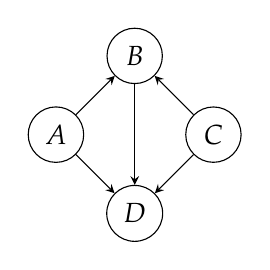
\begin{tikzpicture}
	\node[lightstyle, minimum size=20] (a) at (-1,0) {$A$};
	\node[lightstyle, minimum size=20] (b) at (0,1) {$B$};
	\node[lightstyle, minimum size=20] (c) at (1,0) {$C$};
	\node[lightstyle, minimum size=20] (d) at (0,-1) {$D$};
	\draw[-stealth] (a)--(b);
	\draw[-stealth] (a)--(d);
	\draw[-stealth] (b)--(d);
	\draw[-stealth] (c)--(b);
	\draw[-stealth] (c)--(d);
	\end{tikzpicture}
	\subcaption{}\label{fig:simple_dag}
\end{minipage}
\begin{minipage}[t]{0.4\linewidth}
	\centering
	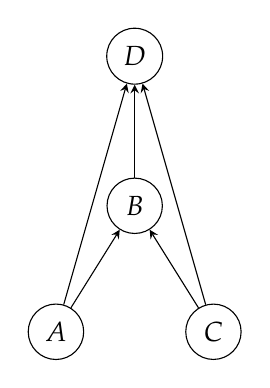
\begin{tikzpicture}
	\node[lightstyle, minimum size=20] (a) at (-1,-1) {$A$};
	\node[lightstyle, minimum size=20] (c) at (1,-1) {$C$};
	\node[lightstyle, minimum size=20] (b) at (0,0.6) {$B$};
	\node[lightstyle, minimum size=20] (d) at (0,2.5) {$D$};
	\draw[-stealth] (a)--(b);
	\draw[-stealth] (a)--(d);
	\draw[-stealth] (b)--(d);
	\draw[-stealth] (c)--(b);
	\draw[-stealth] (c)--(d);
	\end{tikzpicture}
	\subcaption{}\label{fig:simple_layered_dag}
\end{minipage}
\caption{In~\ref{fig:simple_dag}, we see a DAG, and
in~\ref{fig:simple_layered_dag}, the representation of the~DAG as a layered
graph. Notice that the edges~$A \rightarrow D$ and~$C \rightarrow D$ are
manifested as skip connections in the layered
graph.\label{fig:layered_graph_drawing}}
\end{figure}

Any~DAG can be rendered as a layered graph. In a layered graph, nodes are
arranged in horizontal rows, and only vertical connections in one direction,
between nodes in different layers, are allowed. The process by which this is
accomplished is called \emph{layered graph drawing} (see
Figure~\ref{fig:layered_graph_drawing}). Since~$G$ is a~DAG, we can partition
its nodes into an array of successive layers~$L_0, \ldots, L_d$, where~$d$ is
the \emph{depth} of the neural network. The first layer,~$L_0$, consists of the
input nodes ordered from left to right based on the components of~$x$ to which
they correspond. It is called the \emph{input layer}. Not all output nodes
necessarily belong to the last layer, so an \emph{output layer} need not exist
in general. In our case, we assume it does, so~$L_d$ must be the output layer.
Layers in between~$L_0$ and~$L_d$ are called \emph{hidden layers}.
Figure~\ref{fig:two_layer_nn} depicts a small, two-layer neural network.

\begin{figure}
\scriptsize\centering
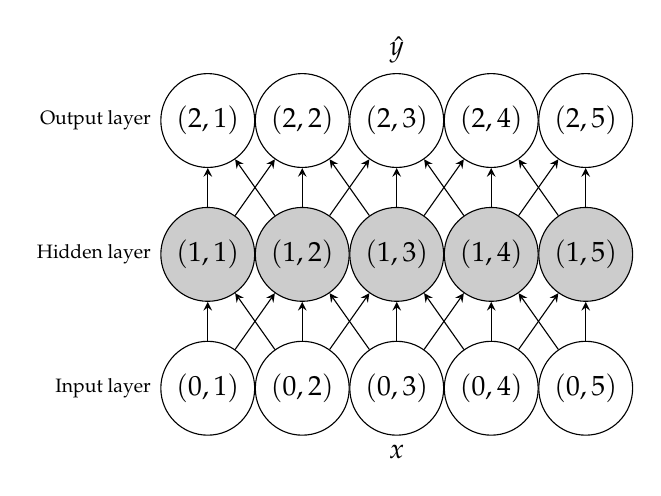
\begin{tikzpicture}

\def\xdist{1.2}
\def\ydist{1.7}

\node[lightstyle, minimum size=20] (a1) at (-2 * \xdist, 0) {$(0, 1)$};
\node[lightstyle, minimum size=20] (a2) at (-1 * \xdist, 0) {$(0, 2)$};
\node[lightstyle, minimum size=20] (a3) at (0, 0)           {$(0, 3)$};
\node[lightstyle, minimum size=20] (a4) at (1 * \xdist, 0)  {$(0, 4)$};
\node[lightstyle, minimum size=20] (a5) at (2 * \xdist, 0)  {$(0, 5)$};

\node[darkstyle, minimum size=20] (b1) at (-2 * \xdist, \ydist) {$(1, 1)$};
\node[darkstyle, minimum size=20] (b2) at (-1 * \xdist, \ydist) {$(1, 2)$};
\node[darkstyle, minimum size=20] (b3) at (0, \ydist)           {$(1, 3)$};
\node[darkstyle, minimum size=20] (b4) at (1 * \xdist, \ydist)  {$(1, 4)$};
\node[darkstyle, minimum size=20] (b5) at (2 * \xdist, \ydist)  {$(1, 5)$};

\node[lightstyle, minimum size=20] (c1) at (-2 * \xdist, 2 * \ydist) {$(2, 1)$};
\node[lightstyle, minimum size=20] (c2) at (-1 * \xdist, 2 * \ydist) {$(2, 2)$};
\node[lightstyle, minimum size=20] (c3) at (0, 2 * \ydist)           {$(2, 3)$};
\node[lightstyle, minimum size=20] (c4) at (1 * \xdist, 2 * \ydist)  {$(2, 4)$};
\node[lightstyle, minimum size=20] (c5) at (2 * \xdist, 2 * \ydist)  {$(2, 5)$};

\node[below] at (0, -0.6) {$x$};
\node[left] at (-2.5 * \xdist, 0) {\scriptsize Input layer};
\node[left] at (-2.5 * \xdist, 1 * \ydist) {\scriptsize Hidden layer};
\node[left] at (-2.5 * \xdist, 2 * \ydist) {\scriptsize Output layer};
\node[above] at (0, 2 * \ydist + 0.6) {$\hat{y}$};

\draw[-stealth] (a1)--(b1);
\draw[-stealth] (a1)--(b2);
\draw[-stealth] (a2)--(b1);
\draw[-stealth] (a2)--(b2);
\draw[-stealth] (a2)--(b3);
\draw[-stealth] (a3)--(b2);
\draw[-stealth] (a3)--(b3);
\draw[-stealth] (a3)--(b4);
\draw[-stealth] (a4)--(b3);
\draw[-stealth] (a4)--(b4);
\draw[-stealth] (a4)--(b5);
\draw[-stealth] (a5)--(b4);
\draw[-stealth] (a5)--(b5);

\draw[-stealth] (b1)--(c1);
\draw[-stealth] (b1)--(c2);
\draw[-stealth] (b2)--(c1);
\draw[-stealth] (b2)--(c2);
\draw[-stealth] (b2)--(c3);
\draw[-stealth] (b3)--(c2);
\draw[-stealth] (b3)--(c3);
\draw[-stealth] (b3)--(c4);
\draw[-stealth] (b4)--(c3);
\draw[-stealth] (b4)--(c4);
\draw[-stealth] (b4)--(c5);
\draw[-stealth] (b5)--(c4);
\draw[-stealth] (b5)--(c5);
\end{tikzpicture}
\caption{A small, two-layer neural network. The pair $(k, j)$ is used to denote
the $j$th unit in layer $k$.\label{fig:two_layer_nn}}
\end{figure}

Computation in a neural network proceeds from layer to layer. Nodes in a layer
are called \emph{units}, and edges between units (which must necessarily be from
different layers) are called \emph{connections}. As in
Figure~\ref{fig:simple_layered_dag}, connections between units in nonconsecutive
layers can occur; these are called \emph{skip connections}. Consequently, in
order for information to propagate from~$L_k$ to~$L_{k + 1}$, we may require the
outputs of all units from~$L_0$ to~$L_{k - 1}$. Let~$w \coloneqq |L_k|$ denote
the \emph{width} of~$L_k$. Rather than thinking about~$L_k$ as a subgraph
of~$G$, we associate~$L_k$ with a vector~$z_k \in \reals{w}$. The value of
component~$z_{ki}$ is given by the output of the of the~$i$th unit from the left
end of~$L_k$. It is now evident that the vector~$x$ is transformed
into~$\hat{y}$ by a series of successive functions~$\sigma_1, \ldots, \sigma_d$
given by
\begin{align}
\begin{split}
	x \eqqcolon z_0 &\xmapsto{\sigma_1} z_1 \\
	(z_0, z_1) &\xmapsto{\sigma_2} z_2 \\
	(z_0, z_1, z_2) &\xmapsto{\sigma_3} z_3 \\
	\vdots\hspace{0.8cm} &\hphantom{\mapsto{\sigma_3}} \vdots \\
	(z_0, \ldots, z_{d - 1}) &\xmapsto{\sigma_d} z_d \coloneqq \hat{y},
\end{split}
\label{eq:forward_propagation}
\end{align}
where $\sigma_k$ is realized by the units in $L_k$.

\begin{figure}[t]
\scriptsize\centering
\begin{tikzpicture}
\node[lightstyle, minimum size=40] (a) at (-4,2) {$(k - 1, 1)$};
\node[lightstyle, minimum size=40] (b) at (-4,0) {$(k - 1, 2)$};
\node[lightstyle, minimum size=40] (c) at (-4,-2) {$(k - 1, 3)$};
\node[lightstyle, minimum size=40] (d) at (0,0) {$(k, 1)$};
\node[draw, right, align=left] (activation) at (1.5, 0) {
	$\begin{alignedat}{2}
	a_{k1} = \;&\weight{(k - 1, 1)}{k1} z_{k - 1, 1} \;+&& \\
		&\weight{(k - 1, 2)}{k1} z_{k - 1, 2} \;+&& \\
		&\weight{(k - 1, 3)}{k1} z_{k - 1, 3} \;+&&\; b_{k1} \\
	\end{alignedat}$\\[\medskipamount]
	$z_{k1} = u_{k1}(a_{k1})$
};

\draw[-stealth] (a) -- node[sloped, above] {$\weight{(k - 1, 1)}{k1}$} (d);
\draw[-stealth] (b) -- node[sloped, above] {$\weight{(k - 1, 2)}{k1}$} (d);
\draw[-stealth] (c) -- node[sloped, above] {$\weight{(k - 1, 3)}{k1}$} (d);
\end{tikzpicture}

\caption{An illustration how the output of~$(k, 1)$, a unit with three inputs
from~$L_{k - 1}$, is computed. In this case, $\parents(k, 1) = \{(k - 1, 1), (k
- 1, 2), (k - 1, 3)\}$. First, the activation~$a_{k1}$ is computed by forming a
linear combination of the outputs of the units in~$\parents(k, 1)$ with the
corresponding weights to~$(k, j)$, and adding the bias~$b_{k1}$. Then, the
output~$z_{k1}$ is determined by applying the activation function~$u_{k1}$
to~$a_{k1}$.\label{fig:unit_output}}
\end{figure}

The~$j$th unit in the input layer of a neural network simply returns the
corresponding component~$x_j$ of the input vector~$x$. On the other hand, each
unit in the hidden and output layers forms a linear combination of the inputs
from previous layers to which it is connected, and adds a bias parameter to the
result. Suppose that~$L_k$ is not the input layer, so that~$k > 0$. The~$j$th
unit in~$L_k$ is denoted by~$(k, j)$, and its activation~$a_{kj}$ is defined as
\begin{equation}
	a_{kj} \;\coloneqq \sum_{(l, i) \in \parents(k, j)} \weight{li}{kj} z_{li} + b_{kj}.
	\label{eq:activation}
\end{equation}
Here,~$\parents(k, j)$ denotes the parents of~$(k, j)$, which are the units that
have edges directed toward~$(k, j)$. This notation allows us to easily
generalize our discussion to layered networks that incorporate skip connections.
The number~$\weight{li}{kj}$ is the \emph{weight} associated with the
connection~$(l, i) \rightarrow (k, j)$, and $b_{kj}$ the \emph{bias} associated
with $(k, j)$. The quantity~$z_{li}$ is the output of unit~$(l, i)$, and is
obtained by applying the unit's \emph{activation function} $u_{li} : \reals{1}
\to \reals{1}$ to the unit's activation~$a_{li}$:
\begin{equation}
	z_{li} = u_{li}(a_{li}).
	\label{eq:output}
\end{equation}
Figure~\ref{fig:unit_output} shows how the activation of a unit with three
parents is computed.

The process of computing the output vector~$z_k$ corresponds to applying the
function~$\sigma_k$. If~$w \coloneqq |L_k|$, then writing
\[
	(z_0, \ldots, z_{k - 1}) \xmapsto{\sigma_k} z_k
\]
is shorthand for saying that we compute~$z_k$ through~$w$ simultaneous
applications of~(\ref{eq:activation}), followed by~$w$ simultaneous
applications of~(\ref{eq:output}). In order to compute the network's
prediction~$\hat{y} \in \reals{m}$ corresponding to an input~$x \in \reals{n}$,
we apply the functions~$\sigma_1, \ldots, \sigma_d$ as described
by~(\ref{eq:forward_propagation}). This process is called \emph{forward
propagation}.

\subsection{Activation Functions and Feature Learning}
\label{sec:act_func_and_feature_learning}

\begin{figure}[t]
\centering
\begin{subfigure}{0.4\textwidth}
	\centering
	\resizebox{!}{4cm}{%
	\begin{tikzpicture}
	\begin{axis}[
		xmin=-4,
		xmax=4,
		xlabel=$x$,
		ylabel=$y$
	]
	\addplot[mark=none, samples=100] {1.7159 * tanh(2 * x / 3)};
	\end{axis}
	\end{tikzpicture}}
	\caption{Plot of $f(x) \coloneqq a \tanh(b x)$, where $a \coloneqq
	1.7159$ and $b \coloneqq 2/3$.\label{fig:tanh_plot}}
\end{subfigure}\hspace{0.5cm}%
\begin{subfigure}{0.4\textwidth}
	\centering
	\resizebox{!}{4cm}{%
	\begin{tikzpicture}
	\begin{axis}[
		xmin=-4,
		xmax=4,
		xlabel=$x$,
		ylabel=$y$
	]
	\addplot[mark=none, samples=1000] {max(0, x)};
	\end{axis}
	\end{tikzpicture}}
	\caption{Plot of $f(x) \coloneqq \max(0,
	x)$.\newline\label{fig:linear_threshold_plot}}
\end{subfigure} \\
\begin{subfigure}{0.4\textwidth}
	\centering
	\resizebox{!}{4cm}{%
	\begin{tikzpicture}
	\begin{axis}[
		xmin=-4,
		xmax=4,
		xlabel=$x$,
		ylabel=$y$
	]
	\addplot[mark=none, samples=100] {4 * 2/3 * 1.7159 * (cosh(2 * x / 3))^2
	/ (cosh(4 * x / 3) + 1)^2};
	\end{axis}
	\end{tikzpicture}}
	\caption{Plot of the derivative of the function
	in~\ref{fig:tanh_plot}.\label{fig:tanh_der_plot}}
\end{subfigure}\hspace{0.5cm}%
\begin{subfigure}{0.4\textwidth}
	\centering
	\resizebox{!}{4cm}{%
	\begin{tikzpicture}
	\begin{axis}[
		xmin=-4,
		xmax=4,
		xlabel=$x$,
		ylabel=$y$
	]
	\addplot[mark=none, samples=1000] {1/2 * (x/abs(x) + 1)};
	\end{axis}
	\end{tikzpicture}}
	\caption{Plot of the derivative of the function
	in~\ref{fig:linear_threshold_plot}.\label{fig:linear_threshold_der_plot}}
\end{subfigure}
\caption{Plots of two of the most common activation functions and their
derivatives.\label{fig:activation_plots}}
\end{figure}

So far in our discussion, we have avoided making specific choices for the
activation function~$u_{kj} : \reals{1} \to \reals{1}$ associated with unit~$(k,
j)$. Three of the most commonly-used activation functions in the literature are
the identity, scaled $\tanh$, and linear threshold functions (see
Figure~\ref{fig:activation_plots}). (In the neural network literature, linear
threshold functions are called ``rectified linear units''~(ReLU), an instance of
specialized terminology that Mehryar Mohri despises.) Typically, all units in
the same layer are associated with the same activation function. We therefore
drop the redundant second index in the subscript of~$u_{kj}$, and simply refer
to the activation function as~$u_k$.

The choices for the constants~$a$ and~$b$ of the scaled $\tanh$ function are
motivated by several reasons~\citep{lecun-98b}. Firstly, the scaled $\tanh$
function is symmetric and approximately linear about the origin. If the inputs
are decorrelated, our choices for~$a$ and~$b$ cause the variance of the scaled
$\tanh$ function to be close to unity. This accelerates the convergence of
optimization algorithms~(see Section~\ref{sec:pp_and_init}).

Secondly, the choices for these constant helps prevent the \emph{vanishing
gradient problem}. Using these constants causes the second derivative of the
scaled $\tanh$ function to be maximized at~$\pm 1$. This is intentional: $\pm 1$
are the binary target values that are typically used for classification in
practice. Suppose that the asymptotes of the scaled $\tanh$ function had been
at~$\pm 1$ instead of~$\pm a$. Then the weights of the network would drastically
increase, in order to produce the large activation values necessary to drive the
outputs of $\tanh$ function to the target values at its asymptotes.  The
derivative of the scaled $\tanh$ function at these large activation values would
be exponentially small~(see Figure~\ref{fig:tanh_der_plot}). Thus, a
minimization algorithm using derivative information would be liable to ``get
stuck''.

Finally, the choices for these constants allow us to intrepret the output of the
network as a measure of confidence towards its classification. When an input is
near the decision boundary separating instances in two classes, we would like
the network to output a small confidence value to reflect this uncertainty. If
the asymptotes of the scaled $\tanh$ function were at~$\pm 1$, then the large
activation values would force the outputs to one of the two extreme values,
regardless of the certainty of the classification. Our choices for~$a$ and~$b$
avoid this problem.

Unlike the scaled $\tanh$ function, the identity function is typically only used
for regression. One common configuration for regression involves alternating
between layers using the scaled $\tanh$ and identity activation functions. For
classification, we typically only use the $\tanh$ or linear threshold functions.
The adoption of the linear threshold function in the literature is relatively
recent~\citep{nair2010rectified}, but many have found that it drastically
reduces training time and improves generalization when compared to the scaled
$\tanh$ function~\citep{krizhevsky2012imagenet}. Despite these general
guidelines, choosing the best activation functions for a particular problem can
involve a certain degree of experimentation.

One of the principles underlying the effectiveness of neural networks is that of
\emph{hierarchical feature learning}, and is the focus of much of the deep
learning research at NYU. A \emph{feature} is a ``simple'' quantity derived from
the input that is designed to identify one or more of the input's salient
characteristics. For example, suppose that we wish to identify whether a given
black and white image contains a human face. One potential feature is the
difference between the sum of intensities of the pixels in the left half of the
image and that of the right half of the image. In neural networks, a feature is
a subset of activation values that become large when a given pattern is present
in the input. This is a result of the weights and biases of the network being
attuned to presence the pattern.

The success of neural networks in image recognition and acoustic modeling has
been attributed to their ability to learn a \emph{hierarchy} of features. In
these applications, the location of a layer~$L_k$ in the network determines the
relative scale of the patterns in the input captured by the features. In some
sense, the lowest layers of the network ``zoom in'' to the input to capture
low-level, local details, while the highest layers of the network ``zoom out''
to capture overarching, global patterns (see Figure~\ref{fig:cnn_features}). It
is plausible that this phenomenon can occur, since each~$\sigma_k$ synthesizes
the information from layers~$L_0, \ldots, L_{k - 1}$ to produce $z_k$.

\afterpage{%
	\clearpage
	\thispagestyle{empty}
	\newgeometry{top = 0in, left = 0in, right = 0in}
	\begin{figure}[p]
	\centering
	\resizebox{\textwidth}{!}{%
		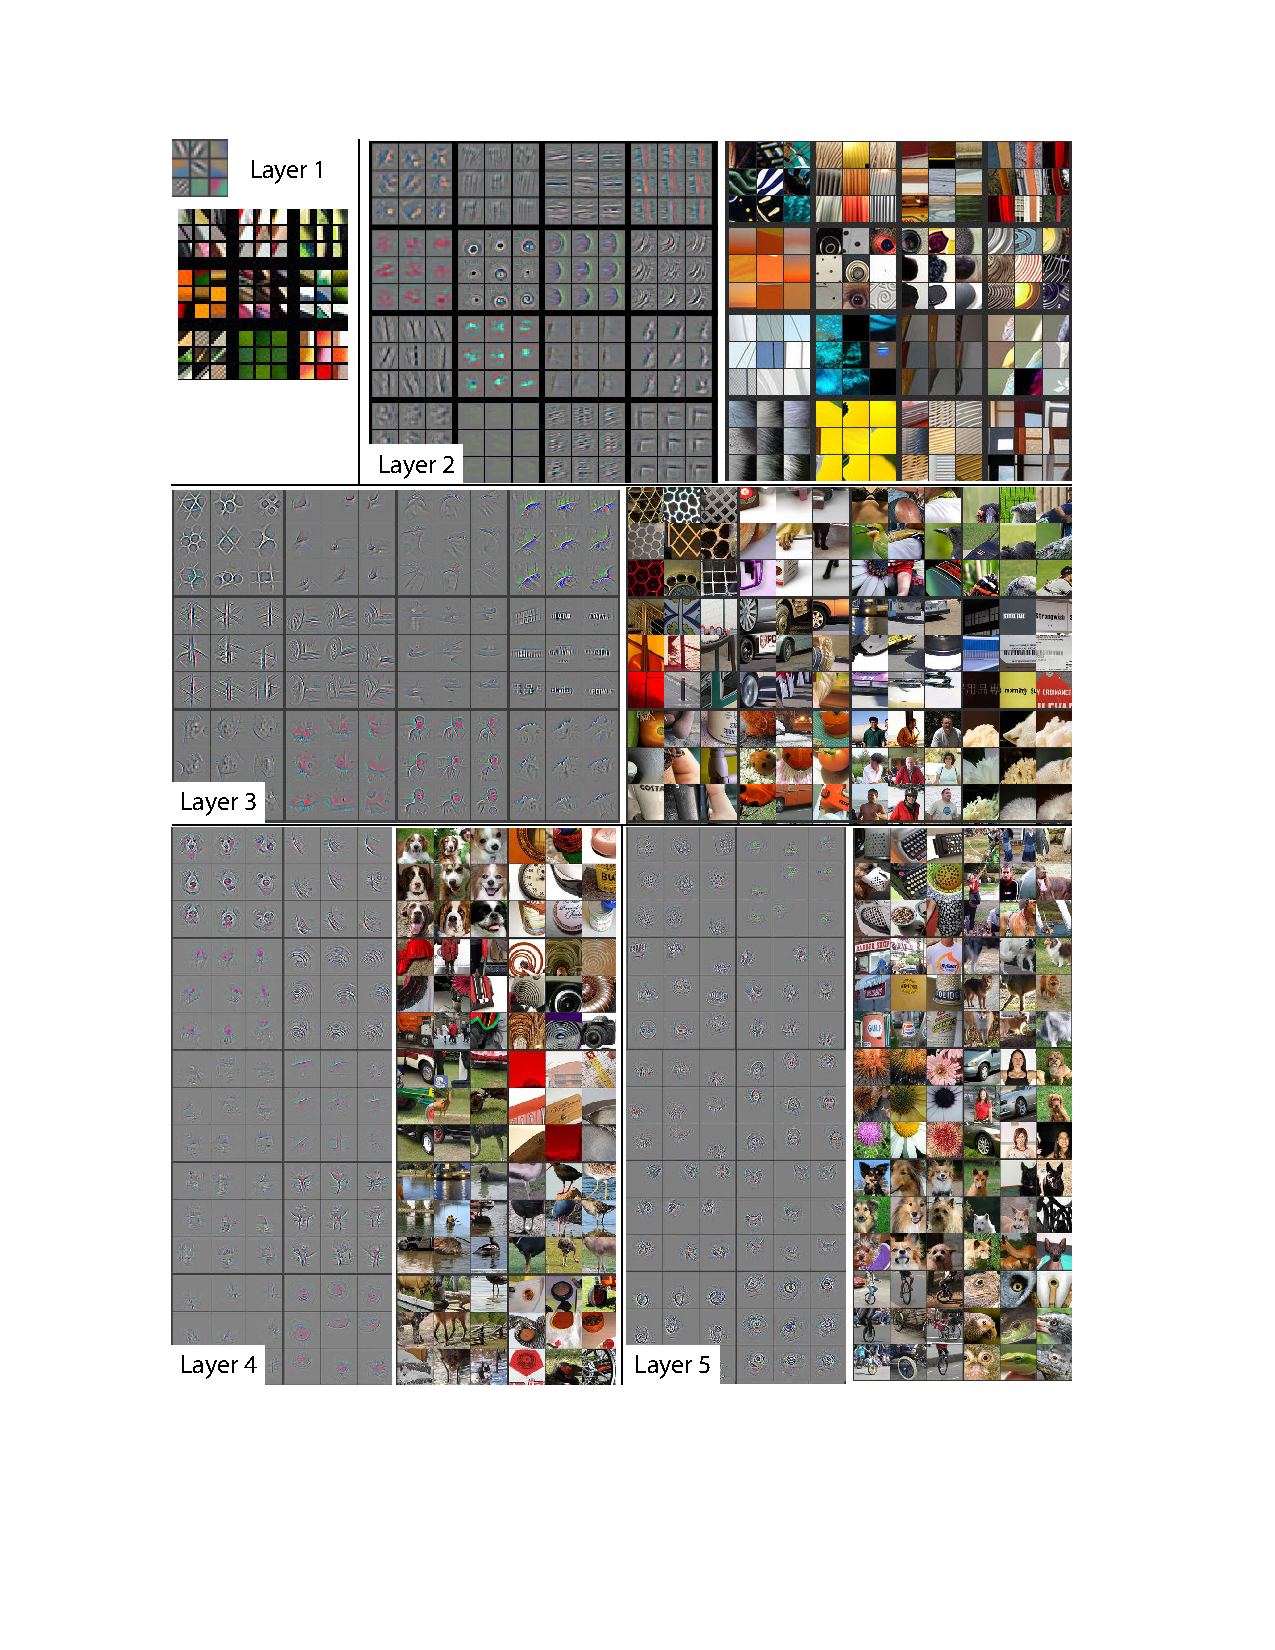
\includegraphics[trim = 0in 1in 0in 0in]{graphics/cnn_features.pdf}
	}
	\begin{minipage}[c]{\textwidth - 2in}
	\caption{Visualization of the hierarchy of features in a fully-trained
	convolutional network for image classification, taken
	from~\citet{zeiler2014visualizing}. For each of the first five layers of
	the network, a selection of the highest activation values in the layer
	is shown alongside the corresponding input images. Note that in general,
	visualizing features in a meaningful way is very difficult.
	\label{fig:cnn_features}}
	\end{minipage}
	\end{figure}
	\restoregeometry
	\clearpage
}

The activation functions discussed so far are useful for learning the low- and
mid-level features in the hierarchy. For learning high-level features,
\emph{radial basis functions}~(RBFs) are sometimes more
appropriate~\citep{lecun-01a}. A radial basis function~$\phi : \reals{1} \to
\reals{1}$ is a continuous function whose value depends only on the
\emph{radius} from a prescribed center~$c \in \reals{n}$. Suppose that we wish
to approximate a function~$f : \reals{n} \to \reals{1}$ whose values at the
points~$c_1, \ldots, c_m$ are known. By centering an~RBF at each~$c_i$, we can
approximate~$f$ using the function $s : \reals{n} \to \reals{1}$ given by
\begin{equation}
	s(x) \coloneqq \sum_{i = 1}^m \lambda_i \phi(\|x - c_i\|_2),
	\label{eq:rbf_sum}
\end{equation}
where~$\lambda \in \reals{m}$ is an adjustable parameter vector. The most
commonly-used RBFs are the Euclidean and Gaussian basis functions. These
functions are given by
\[
	r \mapsto r \quad\text{and}\quad r \mapsto \exp(-k r^2 / 2),
\]
respectively, where~$k \in \reals{+}$.

Since RBFs are used for learning high-level features, they are usually embedded
into one of the topmost layers of the network. As an example, suppose that we
wish to classify~$32 \times 32$ black and white images of handwritten digits
into ten classes, where each class corresponds to a number from zero to nine.
Suppose that~$L_k$ is a layer with~$32^2$ units. By attaching a ten-unit
layer~$L_{k + 1}$ with RBF activation functions to~$L_k$, we can generate ten
scores from~$z_k \in \reals{32 \times 32}$. The~$i$th score is given by~$(z_{k +
1})_i$, and measures the confidence that the input~$x \in \reals{n}$ belongs to
the~$i$th class.

The idea is to get~$z_k$ to match a \emph{prototype} for one of the classes as
closely as possible. We can view the functions~$\sigma_1, \ldots, \sigma_k$ as
nonlinearly deconstructing and reassembling~$x$ to match one of these
prototypes. The ten prototypes~$c_1, \ldots, c_{10}$, are initialized by running
a clustering algorithm, such as~$k$-means, on the training sample. Each
prototype is treated as the center of an~RBF, and is subsumed into the weights
of the network. The proximity of $z_k$ to the $i$th prototype $c_i$ is given by
$\phi(\|x - c_i\|)$, and is a measure of confidence that $x$ belongs to the
$i$th class.

If~$\phi$ is a \emph{normalized RBF}, then the confidence scores are
probabilities. A normalized RBF~$\phi$ is the normalized form of another basis
function~$\psi$. Hence, the $i$th RBF is given by
\begin{equation}
	\phi(x) \coloneqq \frac{\psi(\|x - c_i\|)}
		{\sum_{j = 1}^{10} \psi(\|x - c_j\|)}.
	\label{eq:normalized_rbf}
\end{equation}
Now the ten outputs,~$\phi(\|x - c_i\|)$, $i \in [1, 10]$, form a discrete
probability distribution over the classes.

\subsection{Classification and Regression}

We have seen that a neural network is a biologically-inspired nonlinear function
controlled by two adjustable vectors of parameters: the weights $w$ and the
biases~$b$. Now consider a sample~$S \coloneqq \{(x_1, y_1), \ldots, (x_s,
y_s)\}$, where each~$x_k \in \reals{n}$ is an input vector, and each~$y_k$ is
the target vector that we aim to predict when we are given~$x_k$. We focus on
two categories of tasks that we can perform using neural networks:
classification and regression. For regression, we have~$y_k \in \reals{m}$, so
the output layer consists of a single unit.

For classification, two encoding schemes are possible. The first scheme can only
be used for \emph{unary classification}, in which we wish to classify~$x_k$ into
one of several mutually-exclusive classes. In this scheme, each class is
associated with an index, so~$y_k, \hat{y}_k \in \integers{1}$. These values are
called a \emph{place codes}. A special case of unary classification is
\emph{binary classification}, in which we seek to place~$x_k$ into one of two
mutually-exclusive classes. When using place codes, the output layer consists of
a single unit.

The second scheme can be used for unary classification as well as
\emph{multiclass classification}, in which the~$x_k$ can belong to one or more
classes. This time,~$y_k \in \{0, 1\}^m$ and $\hat{y}_k \in \reals{m}$. These
values are called \emph{distributed codes}. The component!$(y_k)_i$ is one
if~$x_k$ belongs to the $i$th class, and zero otherwise. On the other hand,
$(\hat{y}_k)_i$ is a measure of confidence that $x_k$ belongs to the the $i$th
class. Whether a larger value indicate increased or decreased confidence varies
based on convention.

Distributed codes possess the advantage that they scale well to large
numbers of classes, while place codes do not~\citep{lecun-98b}. When using place
codes, the single output unit of the network must assume one of finitely many
values. If a large number of classes occur with nontrivial probabilities, then
each unit in the penultimate layer of the network must generate an output close
to zero almost all of the time. This becomes increasingly difficult as the
number of classes grows.

\subsection{The Loss Function}

\begin{figure}
\scriptsize\centering
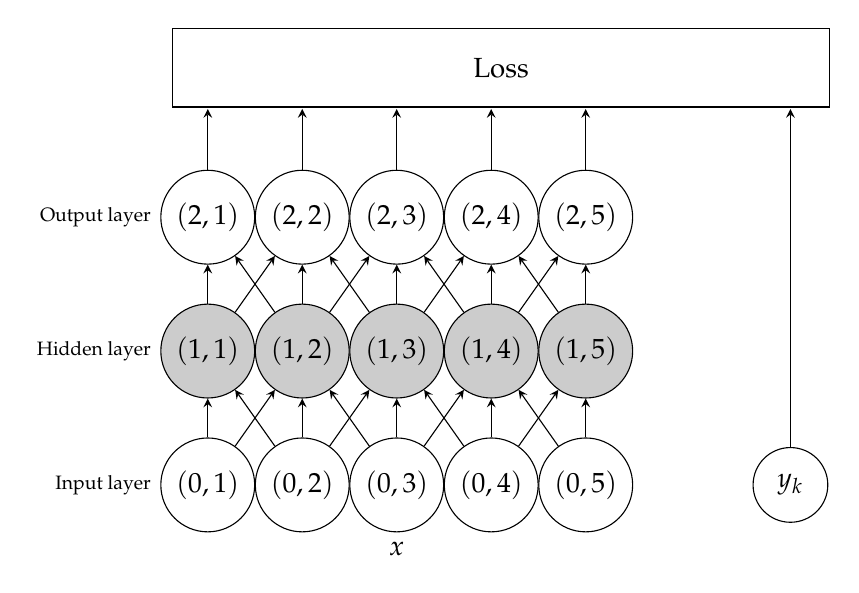
\begin{tikzpicture}

\def\xdist{1.2}
\def\ydist{1.7}

\node[lightstyle, minimum size=20] (a1) at (-2 * \xdist, 0) {$(0, 1)$};
\node[lightstyle, minimum size=20] (a2) at (-1 * \xdist, 0) {$(0, 2)$};
\node[lightstyle, minimum size=20] (a3) at (0, 0)           {$(0, 3)$};
\node[lightstyle, minimum size=20] (a4) at (1 * \xdist, 0)  {$(0, 4)$};
\node[lightstyle, minimum size=20] (a5) at (2 * \xdist, 0)  {$(0, 5)$};

\node[darkstyle, minimum size=20] (b1) at (-2 * \xdist, \ydist) {$(1, 1)$};
\node[darkstyle, minimum size=20] (b2) at (-1 * \xdist, \ydist) {$(1, 2)$};
\node[darkstyle, minimum size=20] (b3) at (0, \ydist)           {$(1, 3)$};
\node[darkstyle, minimum size=20] (b4) at (1 * \xdist, \ydist)  {$(1, 4)$};
\node[darkstyle, minimum size=20] (b5) at (2 * \xdist, \ydist)  {$(1, 5)$};

\node[lightstyle, minimum size=20] (c1) at (-2 * \xdist, 2 * \ydist) {$(2, 1)$};
\node[lightstyle, minimum size=20] (c2) at (-1 * \xdist, 2 * \ydist) {$(2, 2)$};
\node[lightstyle, minimum size=20] (c3) at (0, 2 * \ydist)           {$(2, 3)$};
\node[lightstyle, minimum size=20] (c4) at (1 * \xdist, 2 * \ydist)  {$(2, 4)$};
\node[lightstyle, minimum size=20] (c5) at (2 * \xdist, 2 * \ydist)  {$(2, 5)$};

\node[lightstyle, minimum size=27] (target) at (5, 0) {$y_k$};

\draw (-2.85, 4.8) rectangle (5.5, 5.8) node[fitting node] (loss) {};
\draw (1.325, 5.3) node {Loss};

\node[below] at (0, -0.6) {$x$};
\node[left] at (-2.5 * \xdist, 0) {\scriptsize Input layer};
\node[left] at (-2.5 * \xdist, 1 * \ydist) {\scriptsize Hidden layer};
\node[left] at (-2.5 * \xdist, 2 * \ydist) {\scriptsize Output layer};
%\node[above] at (0, 2 * \ydist + 0.6) {$\hat{y}$};

\draw[-stealth] (a1)--(b1);
\draw[-stealth] (a1)--(b2);
\draw[-stealth] (a2)--(b1);
\draw[-stealth] (a2)--(b2);
\draw[-stealth] (a2)--(b3);
\draw[-stealth] (a3)--(b2);
\draw[-stealth] (a3)--(b3);
\draw[-stealth] (a3)--(b4);
\draw[-stealth] (a4)--(b3);
\draw[-stealth] (a4)--(b4);
\draw[-stealth] (a4)--(b5);
\draw[-stealth] (a5)--(b4);
\draw[-stealth] (a5)--(b5);

\draw[-stealth] (b1)--(c1);
\draw[-stealth] (b1)--(c2);
\draw[-stealth] (b2)--(c1);
\draw[-stealth] (b2)--(c2);
\draw[-stealth] (b2)--(c3);
\draw[-stealth] (b3)--(c2);
\draw[-stealth] (b3)--(c3);
\draw[-stealth] (b3)--(c4);
\draw[-stealth] (b4)--(c3);
\draw[-stealth] (b4)--(c4);
\draw[-stealth] (b4)--(c5);
\draw[-stealth] (b5)--(c4);
\draw[-stealth] (b5)--(c5);

\path
	let
		\p1 = (c1),
		\p2 = (c2),
		\p3 = (c3),
		\p4 = (c4),
		\p5 = (c5),
		\p6 = (target),
		\p7 = (loss.south)
	in
		node (d1) at (\x1, \y7 + 3) {}
		node (d2) at (\x2, \y7 + 3) {}
		node (d3) at (\x3, \y7 + 3) {}
		node (d4) at (\x4, \y7 + 3) {}
		node (d5) at (\x5, \y7 + 3) {}
		node (d6) at (\x6, \y7 + 3) {};

\draw[-stealth] (c1)--(d1);
\draw[-stealth] (c2)--(d2);
\draw[-stealth] (c3)--(d3);
\draw[-stealth] (c4)--(d4);
\draw[-stealth] (c5)--(d5);
\draw[-stealth] (target)--(d6);
\end{tikzpicture}
\caption{A visualization of how the $k$th instance~$(x_k, y_k)$ is fed into the
two-layer neural network from
Figure~\ref{fig:two_layer_nn}.\label{fig:nn_with_loss}}
\end{figure}

Our goal is now to formulate the objective for the minimization algorithm used
to adjust the weights and biases. To do this, we need a function that measures
how well the network's prediction~$\hat{y}_k \in \reals{m}$ for $x_k \in
\reals{n}$ matches the target value~$y_k \in \reals{m}$. This function is called
the \emph{loss function} or \emph{cost function} (see
Figure~\ref{fig:nn_with_loss}). The choice of the loss function depends on the
type of problem we would like to solve.

One way to arrive at the loss function is to assign a probabilistic
interpretation to the network outputs~\citep{ml_bishop}. Let~$w$ and~$b$ be the
vectors of weights and biases of the network. By choosing an explicit
representation for the conditional distribution~$p(y_k \given x_k, w, b)$, we
are led to a canonical loss function corresponding to this choice. Let~$X =
\{x_1, \ldots, x_s\}$ and~$Y = \{y_1, \ldots, y_s\}$. If we assume that the
instances~$(x_k, y_k) \in S$ are iid, then we can apply the chain rule to write
\[
	p(Y \given X, w, b) = \prod_{k = 1}^s p(y_k \given x_k, w, b).
	\label{eq:likelihood_function}
\]
The LHS of~(\ref{eq:likelihood_function}) is called the likelihood function. The
canonical loss function is obtained by maximizing the likelihood function over
the~$w$ and~$b$. Maximizing the likelihood function is equivalent to minimizing
its negative logarithm, which is given by
\begin{equation}
	-\ln{p(Y \given X, w, b)} = -\sum_{k = 1}^s \ln{p(y_k \given x_k, w, b)}.
	\label{eq:nll}
\end{equation}
The LHS of~(\ref{eq:nll}) is called the negative log-likelihood function~(NLL).

For regression, it is often appropriate to assume that
\[
	p(y_k \given x_k, w, b) = N(y_k \given \hat{y}_k, \beta^{-1}),
\]
where~$N$ is the normal distribution, which for mean~$\mu$ and
variance~$\sigma^2$ is defined as
\[
	N(x \given \mu, \sigma^2) \coloneqq \frac{1}{\sqrt{2 \pi \sigma^2}}
		\exp\left( -\frac{1}{2 \sigma^2} (x - \mu)^2 \right).
\]
The value~$\hat{y}_k$ is the network's prediction for~$x_k$, and~$\beta$ is the
precision (inverse variance) of the Gaussian noise. The corresponding NLL
function is given by
\[
	\frac{\beta}{2} \sum_{k = 1}^s \left(\hat{y}_k - y_k\right)^2 -
		\frac{s}{2} \ln\beta + \frac{s}{2} \ln(2 \pi).
\]
We discard the constant terms, which do not affect the minimization process.
This leaves us with the sum-of-squares loss function, which is given by
\begin{equation}
	E(w, b)
	\coloneqq \frac{1}{2} \sum_{k = 1}^s \left(\hat{y}_k - y_k\right)^2
	= \sum_{k = 1}^s e(\hat{y}_k, y_k),
	\label{eq:sum_of_squares}
\end{equation}
where~$e$ is the per-instance loss function
\[
	e(\hat{y}_k, y_k) \coloneqq \frac{1}{2} \left(\hat{y}_k - y_k\right)^2.
\]

The sum-of-squares error function is generally inappropriate for classification.
We adopt the use of distributed codes, so~$y_k \in \{0, 1\}^m$ and $\hat{y}_k
\in \reals{m}$. We further suppose that the components of~$\hat{y}_k$ determine
a discrete probability distribution over the classes. For convenience, we
define~$y_{ki} \coloneqq (y_k)_i$ and~$\hat{y}_{ki} \coloneqq (\hat{y}_k)_i$.
Our assumption is that the conditional distribution is categorical, and given by
\[
	p(y_k \given x_k, w, b) = \prod_{i = 1}^m \left(\hat{y}_{ki}\right)^{y_{ki}}.
\]
The corresponding NLL function is the \emph{multiclass cross-entropy function},
and does not have any constant terms that we can discard. So we define
\[
	E(w, b)
	= -\sum_{k = 1}^s \sum_{i = 1}^m y_{ki} \ln\hat{y}_{ki}
	= \sum_{k = 1}^s e(\hat{y}_k, y_k),
\]
where~$e$ is the per-instance loss function
\[
	e(\hat{y}_k, y_k) \coloneqq -\sum_{i = 1}^m y_{ki} \ln\hat{y}_{ki}.
\]
In the special case where we are performing binary classification, with~$y_k \in
\{0, 1\}$ and~$\hat{y}_k \in \reals{1}$, we can write
\[
	p(y_k \given x_k, w, b) = \left(\hat{y}_k\right)^{y_k}
		\left(1 - \hat{y}_k\right)^{1 - y_k}
\]
and
\[
	e(\hat{y}_k, y_k) \coloneqq -\big(
		y_k \ln\hat{y}_k + (1 - y_k) \ln(1 - \hat{y}_k) \big).
\]

The cross-entropy loss function is almost exclusively used with a special
activation function for the output layer of the network. This activation
function is the \emph{softmax} function; for~$z \in \reals{m}$, it is given by
\begin{equation}
	\phi(z_i) = \frac{\exp(z_i)}{\sum_{j = 1}^m \exp(z_j)}.
	\label{eq:softmax}
\end{equation}
This is a normalized RBF of the form given by~(\ref{eq:normalized_rbf}). It
follows that using~(\ref{eq:softmax}) as the output activation function will
guarantee that the components of~$\hat{y}_k$ determine a discrete probability
distribution over the classes. For binary classification, (\ref{eq:softmax})
reduces to the \emph{logistic sigmoid} function upon setting the
component~$\hat{y}_{k2}$, which corresponds to the second class, to zero:
\begin{align*}
	\phi(\hat{y}_1)
	&= \frac{\exp(\hat{y}_1)}{\exp(\hat{y}_1) + \exp(\hat{y}_2)} \\
	&= \frac{\exp(\hat{y}_1)}{\exp(\hat{y}_1) + 1} \\
	&= \frac{1}{1 + \exp(-\hat{y}_1)}.
\end{align*}
Thus, the softmax function can be viewed as a generalization of the logistic
sigmoid function to more than two classes.

\subsection{Data Preprocessing and Initialization}
\label{sec:pp_and_init}

Preprocessing the data can have drastic effects on convergence of the
optimization algorithm used for learning. However, normalizing the features (the
components of an input~$x_k \in \reals{n}$) must be done with great care, so as
not to destroy useful information encoded by the relative magnitudes of a
feature. Suppose that it is equally important that we predict the target value
for any input~$x_k$ from our training sample~$D$. This is \emph{not} the case,
for instance, when we wish to predict whether the person corresponding to an
input~$x_k$ has a rare disease. Then it can be beneficial to center and scale
the features by subtracting the mean vector~$\mu$ and scaling by the variance
vector~$\sigma$. Specifically, each input~$x_k$ is normalized by computing
\begin{equation}
	\bar{x}_k \coloneqq \frac{x_k - \mu}{\sigma}.
	\label{eq:center_and_scale}
\end{equation}

In general, it is recommended to \emph{decorrelate} the features whenever
possible~\citep{lecun-98b}. Doing so decouples the updates to the individual
weights of the network during the optimization process, which accelerates
convergence. \citet{lecun-98b} give an intuitive explanation for why
decorrelating the inputs can be beneficial. Consider the extreme case where all
components of the inputs are positive. Let~$(1, j)$ be a unit in the second
layer of the network, and let~$\tilde{x}_k$ consist of the components of~$x_k$
corresponding to~$\parents{(1, j)}$ (see Figure~\ref{fig:two_layer_nn}).
Let~$\delta$ be the scalar error computed for $(1, j)$ using the techniques
discussed in Section~\ref{sec:computing_derivatives}. Then a na\"{i}ve
first-order optimization algorithm will update the weights to~$(1, j)$ by an
amount proportional to~$\delta \tilde{x}_k$. Thus, the weights to~$(1, j)$ will
either \emph{all} increase or \emph{all} decrease (depending on~$\sign(\delta)$)
after each update. This makes finding a good weight configuration difficult. A
more sophisticated approach to decorrelating the inputs involves
PCA~\citep{lecun-98b, krizhevsky2012imagenet}.

The initial values of the weights can have a significant impact on both
convergence speed and generalization error. Suppose that we use the scaled
$\tanh$ activation function. In order to avoid vanishing gradient problem, we
would like the activation values to remain in the range~$[-1, 1]$, which is
within the linear region of the scaled $\tanh$ function. One way of enforcing
this is to require that the activation values have zero mean and unit
variance~\citep{lecun-98b}.

Suppose that the inputs are centered and scaled according
to~(\ref{eq:center_and_scale}), so that
\[
	\E(x_i) = 0 \quad\text{and}\quad \Var(x_i) = 1,
\]
for each~$i \in [1, n]$. From~(\ref{eq:activation}), we know that the activation
of~$(1, j)$ is given by
\[
	a_{1j} \;\coloneqq \sum_{(0, i) \in \parents(1, j)} \weight{0l}{1j} x_{0l} + b_{1j}.
\]
If the weights are chosen independently from the inputs, and both the weights
and the biases have zero mean, then we have
\begin{align*}
	\E(a_{1j})
	&= \E\Bigg(\sum_{(0, i) \in \parents(1, j)} \weight{0l}{1j} x_{0l} + b_{1j}\Bigg) \\
	&= \sum_{(0, i) \in \parents(1, j)} \E(\weight{0l}{1j} x_{0l} + b_{1j}) \\
	&= \sum_{(0, i) \in \parents(1, j)} \left(\E(\weight{0l}{1j} x_{0l}) + \E(b_{1j})\right) \\
	&= \sum_{(0, i) \in \parents(1, j)} \E(\weight{0l}{1j}) \E(x_{0l}) = 0.
\end{align*}
Thus, our requirement that the activation values have zero mean is satisfied.

We now describe how to enforce that~$\Var(a_{1j}) = 1$. Let $f \coloneqq
|\text{Pa}(1, j)|$, and suppose that all weights have the same standard
deviation~$\sigma$. The value~$f$ is called the \emph{fan-in} of~$(1, j)$. To
solve for the value of~$\sigma$ that forces~$\Var(a_{1j}) = 1$, we compute
\begin{align*}
	\Var(a_{1j})
	&= \Var\Bigg(\sum_{(0, i) \in \parents(1, j)} \weight{0l}{1j} x_{0l} + b_{1j}\Bigg) \\
	&= \Var\Bigg(
		\sum_{(0, i) \in \parents(1, j)} \weight{0l}{1j} x_{0l} +
		\sum_{(0, i) \in \parents(1, j)} b_{1j}
	\Bigg) \\
	&= \Var\Bigg(\sum_{(0, i) \in \parents(1, j)} \weight{0l}{1j} x_{0l}\Bigg)\\
	&= \sum_{(0, i) \in \parents(1, j)} \left(
		\Var(\weight{0l}{1j}) \Var(x_{0l}) -
		\E(\weight{0l}{1j})^2 \E(x_{0l})^2
	\right) \\
	&= \sum_{(0, i) \in \parents(1, j)} \Var(\weight{0l}{1j}) \Var(x_{0l}) \\
	&= \sum_{(0, i) \in \parents(1, j)} \sigma^2 = f \sigma^2.
\end{align*}
So in order to enforce that $\Var(a_{1j}) = 1$, we should sample the weights
from a distribution with zero mean and standard deviation given by
\[
	\sigma = \frac{1}{\sqrt{f}}.
\]
The most common choices of distribution for weight initialization are the
uniform and normal distributions~\citep{lecun-98b, krizhevsky2012imagenet}.

The training dynamics of neural networks are vitally important but poorly
understood. As the weights and biases of the network are calibrated using the
minimization algorithm, the distributions of the activation values at each layer
evolve. For deep networks with many layers, the vanishing gradient problem is
greatly compounded. In particular, the greater the depth of a layer in the
network, the greater the tendency of the activation values to cluster around
zero or become very large~\citep{glorot2010understanding}. This causes the
vanishing gradient problem discussed in
Section~\ref{sec:act_func_and_feature_learning}. The subtle numerical issues
resulting from these complex interactions largely determines whether, when, and
how a given minimization algorithm will converge.

The use of a good weight initialization scheme can help mitigate the undesirable
saturation of the activation values~\citep{glorot2010understanding}. Several
authors have recently proposed new initialization schemes that they found were
more effective than the one given here~\citep{glorot2010understanding,
martens2010deep}. Another strategy is to incorporate a form of internal
normalization into the network by adding \emph{local response normalization}
layers~\citep{krizhevsky2012imagenet}. Part of the reason that training deep
neural networks is so difficult is that these dynamics are so poorly understood.
Development of a deeper understanding of what is happening in these situations
is likely to have widespread practical consequences.

\subsection{Computing Derivatives}
\label{sec:computing_derivatives}

TODO

\subsection{Convolutional Networks}

TODO

\section{Concepts from Statistical Learning Theory}

\subsection{Generalization and PAC-learning}

Our initial goal when motivating the discussion for neural networks was to
``learn'' what a given function~$f: \reals{n} \to \reals{m}$ does to
transform~$x \in \reals{n}$ to~$y \in \reals{m}$. But what exactly does it mean
to learn? So far, we have neglected to provide a definition for what it means
for an algorithm ``learn'' a model to solve a given problem. A rigorous
definition for learning is given in the field of statistical learning theory.
This definition will have widespread consequences in shaping our criteria used
to determine when an optimization algorithm is good.

When performing binary classification, each training instance~$(x_k, y_k) \in S$
is implicitly associated with a target \emph{concept} that we wish to learn.
This concept is a mapping~$c$ from the input space~$X$ to the output space~$Y
\coloneqq \{0, 1\}$, such that~$y_k = c(x_k)$. The set of all concepts
associated with our classification task is called the \emph{concept class}, and
is denoted by~$C$. A concept can be something simple, such as the set of
axis-aligned rectangles in~$\reals{2}$, or something exceedingly complex, such
as the manifold of human faces in~$\reals{256 \times 256}$, the space of~$256
\times 256$ black and white images. We assume that all instances are drawn iid
from some unknown distribution~$D$~over~$X$.

Suppose that we are given a family of candidate functions~$F$, such that~$f : X
\to \{0, 1\}$ for every~$f \in F$. The task of our learning algorithm is to
minimize the probability of a misclassification from an instance~$x \sim D$.
This leads to the following definition for \emph{generalization error}.

\begin{definition}[Generalization error~\citep{ml_mohri}]
Given a candidate function~$f \in F$, a target concept~$c \in C$, and an
underlying distribution~$D$, the \emph{generalization error} or \emph{risk}
of~$f$ is defined as
\[
	R(f) \coloneqq \Pr_{x \sim D}(f(x) \neq c(x)) =
		\E_{x \sim D} \left(\ind{f(x) \neq c(x)}\right).
\]
\end{definition}

The generalization error is not a quantity that we can directly measure.
Instead, we must work with the \emph{empirical error}, the average number of
misclassifications over our training sample~$S \sim D$.

\begin{definition}[Empirical error~\citep{ml_mohri}]
Given a candidate function~$f \in F$, a target concept~$c \in C$, and a
sample~$S \coloneqq \{(x_1, y_k), \ldots, (x_s, y_s)\} \sim D$, the
\emph{empirical error} or \emph{empirical risk} of~$f$ is defined as
\[
	\hat{R}(f) \coloneqq \frac{1}{s} \sum_{i = 1}^s \ind{f(x) \neq c(x)}.
\]
\end{definition}

There is a simple relationship between the empirical and generalization errors.
Let~$f \in F$. Using the linearity of expectations and the fact that~$S$ is
drawn iid from~$D$, it is easy to show that
\[
	\E_{S \sim D} (\hat{R}(f)) = R(f).
\]
In other words, the generalization error of~$f$ is simply the average
misclassification rate over samples drawn from~$D$. We are now ready to present
the the definition of probably approximate correct~(PAC) learning.

\begin{definition}[PAC-learning~\citep{ml_mohri}]
Suppose that we are performing binary classification of inputs from an input
space~$X$, and let~$C$ be the associated concept class. Let~$O(n)$ be an upper
bound on the space complexity of an input~$x \in X$. Given an algorithm~$A$ and
a sample~$S \sim D$, let~$f_S \in F$ denote the candidate function found by~$A$
for~$S$. Then~$C$ is PAC-learnable if there exists an algorithm~$A$ and a
polynomial function~$g : \reals{4} \to \reals{1}$ such that for any~$\epsilon,
\delta \in (0, 1]$, for all distributions~$D$~over~$X$, and for any target
concept~$c \in C$, the following holds for any sample~$S \sim D$ of size~$s \geq
g(1/\epsilon, 1/\delta, n, \size(c))$:
\[
	\Pr_{S \sim D} (R(f_S) \leq \epsilon) \geq 1 - \delta.
\]
If $A$ runs in~$g(1/\epsilon, 1/\delta, n, \size(c))$, then~$C$ is said to be
efficiently PAC-learnable. In this case, $A$~is called a PAC-learning algorithm
for~$C$.
\end{definition}

The definition for PAC-learning is verbose, but the underlying intuition is
simple. Suppose that we have a target generalization error~$\epsilon$ that we
wish to attain with probability~$1 - \delta$ on any sample~$S \sim D$. Then~$C$
is PAC-learnable if the sample size required to meet our goals is bounded by a
polynomial function of~$1/\epsilon$ and~$1/\delta$. Roughly speaking, $A$ must
find a function in~$F$ that is \emph{approximately correct} with \emph{high
probability}. But it must be able to do this using a sample size that is not
``too large''. The extension of space and time complexity to sample size
requires this notion of ``high probability''.

One of the goals of statistical learning theory is to derive upper bounds on the
generalization error in various situations. When such an upper bound applies to
the particular situation at hand, we know that it is possible, at least in
principle, to learn efficiently. Many of these upper bounds take the following
form. Let~$\delta \in (0, 1]$ be our target confidence, and let~$s$ be the size
of the training samples drawn from~$D$. Then with probability~$1 - \delta$, it
holds for any~$f \in F$ that
\begin{equation}
	R(f) \leq \hat{R}(f) + c \sqrt{\frac{\capacity(F)}{s}},
	\label{eq:generalization_bound}
\end{equation}
where~$c \in \reals{+}$ and~$\capacity(F)$ is a quantity that measures the
complexity of our chosen family of functions. When we apply the
bound~(\ref{eq:generalization_bound}), we often subsume auxiliary constants
into~$c$. So two occurrences of~$c$ do not necessary represent the same constant
value.

\subsection{ERM vs SRM}
\label{sec:erm_vs_srm}

The central idea of statistical learning theory is that learning is a tradeoff
between minimizing the training error and the complexity of the family of
functions used to model~$C$. These quantities correspond to the first and second
terms on the RHS of~(\ref{eq:generalization_bound}), respectively. This tradeoff
can be expressed in another way that is particularly illuminating. Let
\[
	f^\star \coloneqq \argmin_{f} R(f) \quad\text{and}\quad
	f_F^\star \coloneqq \argmin_{f \in F} R(f).
\]
In other words, $R(f^\star)$~is the best we can ever hope to do, while
$R(f_F^\star)$~is the best we can do using our chosen family $F$. Given a
function~$f \in F$, we define the \emph{excess error}~$\mathcal{E}$ as
\begin{equation}
	\mathcal{E} \coloneqq R(f) - R(f^\star)
		= (R(f_F^\star) - R(f^\star)) + (R(f) - R(f_F^\star))
		= \apperr + \esterr,
	\label{eq:app_est_decomp}
\end{equation}
where
\[
	\apperr = R(f_F^\star) - R(f^\star)
	\quad\text{and}\quad
	\esterr = R(f) - R(f_F^\star)
\]
The quantity~$\apperr$ is called the \emph{approximation error}, and measures
how well functions in~$F$ can approximate functions in~$C$. It is generally
intractible, as we have no way of estimating it. The quantity~$\esterr$ is
called the \emph{estimation error}, and measures the performance of~$f$ relative
to that of the best-in-class hypothesis~$f_F^\star$. It is easy to show
that~$\esterr$ is bounded above by the second term on the RHS
of~(\ref{eq:generalization_bound}). Equation~\ref{eq:app_est_decomp} tells us
that the quality of a candidate function~$f$ is determined by the sum of these
errors.

Reducing the training error causes the estimation error to decrease, while
reducing the complexity term causes the approximation error to decrease. But
reducing the approximation error often requires increasing $\capacity(F)$, and
this increases the complexity term. On the other hand, reducing the complexity
term requires decreasing $\capacity(F)$, inhibiting our ability to
approximate~$C$. This increases the training error. The interplay between these
two errors is called the \emph{approximation-estimation tradeoff}.

\begin{figure}
\centering
\resizebox{0.6 \textwidth}{!}{%
	\includegraphics{graphics/srm_graph.png}
}
\caption{Visualization of the SRM procedure (adapted from~\citet{ml_mohri}). The
SRM procedure minimizes an upper bound of the generalization error that is a sum
of the training error and the complexity term.\label{fig:srm_graph}}
\end{figure}

Minimizing only the training error while ignoring the complexity term is called
\emph{empirical risk minimization}~(ERM), and is inadvisable on both theoretical
and practical grounds. An alternative procedure that contols $\capacity(F)$ is
called \emph{structural risk minimization}~(SRM). Let~$c \in \reals{+}$, and
define
\begin{equation}
	F_\lambda \coloneqq \{ f \in F : \complexity(f) \leq c \},
	\label{eq:regularized_family}
\end{equation}
where $\complexity(f)$ is a measure of complexity of~$f$. Consequently, $F_a
\subseteq F_b$ whenever~$a, b \in \reals{+}$ such that~$a < b$. ERM~and~SRM seek
to find the functions given by
\begin{equation}
	f_{\text{ERM}} \coloneqq \argmin_{f \in F} \hat{R}(f)
	\quad\text{and}\quad
	f_{\text{SRM}} \coloneqq \argmin_{\substack{c \in \reals{+} \\ f \in F_c}}
		\hat{R}(f),
	\label{eq:erm_srm_solutions}
\end{equation}
respectively. The SRM procedure finds a function in~$F$ that minimizes the
generalization bound~(\ref{eq:generalization_bound}) (see
Figure~\ref{fig:srm_graph}). We can transform second equation
in~(\ref{eq:erm_srm_solutions}) into an unconstrained minimization problem by
using the penalty method. This gives
\begin{equation}
	f_{\text{SRM}} = \argmin_{\substack{\lambda \in \reals{+} \\ f \in F}}
		\left(\hat{R}(f) + \lambda\complexity(f)\right).
	\label{eq:srm_penalty}
\end{equation}
The Lagrange multiplier~$\lambda$ called the the \emph{regularization
parameter}, and penalizes more complex functions. We can now conduct our search
over~$\lambda$ instead of over~$c$. If~$H$ is a vector space, then we can define
$\complexity(f) \coloneqq \|f\|$ for some norm~${\|\cdot\|}$. Note that SRM
involves finding the solution to several ERM subproblems, and is intractible in
general. In practice, we find an approximate SRM solution by using
cross-validation to choose~$\lambda^\star$ from a finite sequence~$\{ \lambda_k
\}_{k = 1}^r$.

As an example, suppose that we are are performing least-squares regression,
where~$X = \reals{n}$ and~$Y \in \reals{1}$. Let~$S$ be a training sample
consisting of~$s$ instances. We define
\[
	F \coloneqq \{ x \mapsto \trans{w}x + b : w \in \reals{n}, b \in
		\reals{1} \},
	\label{eq:affine_family}
\]
and assume let~$E$ be the sum-of-squares error given
by~(\ref{eq:sum_of_squares}). According to the theory developed so far, choosing
$f \coloneqq \argmin_{f \in F} E(f)$ is highly inadvisable. Let $\complexity(f)
\coloneqq \|w\|_2$ for any $f \in F$. A better idea would be to try sequence of
values for~$\lambda$ in~(\ref{eq:srm_penalty}), such as~$\{ \lambda_k \}_{k =
-5}^5$, where~$\lambda_k \coloneqq 2^k$. The results from statistical learning
theory shape our understanding of how we should solve problems in machine
learning.

\section{Characterizing Optimization Algorithms}

\subsection{Goals of Optimization}

We turn our focus to applying statistical learning theory to characterize the
quality of optimization algorithms for machine learning. Let~$f_{\text{ERM}}$ be
given by~(\ref{eq:erm_srm_solutions}). During training, we only require that the
optimization algorithm produce a function~$\hat{f} \in F$, whose empirical error
is within a fixed tolerance~$\rho \in \reals{+}$ of that of~$f_{\text{ERM}}$:
\begin{equation}
	\hat{R}(\hat{f}) - \hat{R}(f_{\text{ERM}}) \leq \rho.
	\label{eq:tol_eq}
\end{equation}
The expectation of the LHS of~(\ref{eq:tol_eq}) taken over a sample~$S \sim D$
is called the \emph{optimization error}~\citep{bousquet2008tradeoffs}, and is
defined as
\[
	\opterr \coloneqq R(\hat{f}) - R(f_{\text{ERM}}).
\]
We can now express the excess error of~$\hat{f}$ as
\begin{align}
	\mathcal{E}
	&= (R(f_F^\star) - R(f^\star)) + (R(f_{\text{ERM}}) - R(f_F^\star)) +
		(R(\hat{f}) - R(f_{\text{ERM}})) \\
	&= \apperr + \esterr + \opterr.
	\label{eq:excess_error}
\end{align}

In practice, the quality of the solution to a machine learning problem is
determined by monetary cost (which determines the maximum sample
size~$s_{\text{max}}$) and human patience (which determines the limit on
computation time~$t_{\text{max}}$). The definition for PAC-learning is one way
of characterizing when one might be satisfied with the performance of a learning
algorithm with respect to these constraints. Let~$t(F, \rho, s)$ represent the
time required by the optimization algorithm to find a function~$\hat{f} \in F$
satisfying~$\opterr \leq \rho$, given a sample of size~$s$. Minimizing the
excess error in~(\ref{eq:excess_error}) subject to the constraints
on~$s_{\text{max}}$ and~$t_{\text{max}}$ yields the following meta-optimization
problem~\citep{bousquet2008tradeoffs}:
\begin{equation}
\begin{aligned}
	& \underset{F, \rho, s}{\text{minimize}} & &
		\mathcal{E} = \apperr + \esterr + \opterr \\
	& \text{subject to} & & \hspace{3.2em} s \leq s_{\text{max}} \\
	& & & t(F, \rho, s) \leq t_{\text{max}}.
\end{aligned}
\label{eq:metaopt_program}
\end{equation}
Table~\ref{tab:metaopt_variables} shows how the errors and computing time are
affected when $\capacity(F)$, $\rho$, and~$s$ are increased.

\begin{table}
\centering
\begin{tabular}{lccc}
\toprule
& $\capacity(F)$ & $s$ & $\rho$ \\
\midrule
$\apperr$ & $\downarrow$ & \text{---} & \text{---} \\
$\esterr$ & $\updownarrow$ & $\updownarrow$ & \text{---} \\
$\opterr$ & $\uparrow$ & $\uparrow$ & $\downarrow$ \\
$t$ & $\uparrow$ & $\uparrow$ & $\downarrow$ \\
\bottomrule
\end{tabular}
\caption{The effects of increasing $\capacity(F)$, $s$, and~$\rho$ on the three
errors and computing time. The symbol $\updownarrow$ indicates that either an
increase or a decrease is possible.\label{tab:metaopt_variables}}
\end{table}

As stated in~\citet{bousquet2008tradeoffs}, ``the solution of the optimization
program~(\ref{eq:metaopt_program}) depends critically on which budget constraint
is active: [the] constraint~$s < s_{\text{max}}$ on the number of examples, or
[the] constraint~$t < t_{\text{max}}$ on the training time''. A
\emph{small-scale} problem is one that is constrained by the sample size. In
this case, the computation time is not limited, so we can make~$\opterr$
negligible by choosing~$\rho$ sufficiently small. Using the fact that~$\esterr$
is bounded above by the second term of~(\ref{eq:generalization_bound}), we have
\begin{equation}
	\mathcal{E} = \apperr + \esterr \leq \apperr + c
		\sqrt{\frac{\capacity(F)}{s}}.
	\label{eq:small_scale_bound}
\end{equation}
Hence minimizing~$\mathcal{E}$ boils down to the discussion in
Section~\ref{sec:erm_vs_srm}. A~\emph{large-scale} problem is one that is
constrained by the maximum computing time. In this case, performing approximate
optimization by choosing~$\rho > 0$ improves generalization, because we can
process more training instances in the allotted time.
Using~(\ref{eq:generalization_bound}), it is easy to show that
\begin{equation}
	\mathcal{E}
	= \apperr + \esterr + \opterr
	\leq \apperr + \rho + c\sqrt{\frac{\capacity(F)}{s}}.
	\label{eq:large_scale_bound}
\end{equation}

Unfortunately, the bounds~(\ref{eq:small_scale_bound})
and~(\ref{eq:large_scale_bound}) are too pessimistic, and do not accurately
reflect reality. In order to proceed with our analysis, we make some simpliyfing
assumptions. First, we assume that $F$~is the family of affine functions given
by~(\ref{eq:affine_family}). In this special case, the generalization
bound~(\ref{eq:generalization_bound}) simplifies to
\[
	R(f) \leq \hat{R}(f) + c \sqrt{\frac{n}{s}}.
\]
A much sharper bound on the excess error can now be
applied~\citep{bousquet2008tradeoffs}. It is given by
\begin{equation}
	\mathcal{E}
	= \apperr + \esterr + \opterr
	\leq c \left( \apperr + \left(\frac{n}{s}\log\frac{s}{n}\right)^\alpha +
		\rho \right),
	\label{eq:fast_rate_bound}
\end{equation}
where~$\alpha \in [1/2, 1]$ is a constant that depends on a variance bound on
the loss function. Since the three components of the excess error should
decrease at approximately the same rate~\citep{bousquet2008tradeoffs}, we make
the additional assumption that
\begin{equation}
	\mathcal{E} \approx \apperr \approx \esterr \approx \opterr \approx
		\left(\frac{n}{s}\log\frac{s}{n}\right)^\alpha \approx \rho.
	\label{eq:error_equiv}
\end{equation}

\subsection{Analysis of Optimization Algorithms}

We now investigate the properties of four specific optimization algorithms.
Assume that our empirical loss function~$E$ is convex and twice differentiable
(e.g. the sum-of-squares loss function). For convenience, we let~$\theta \in
\reals{2n}$, where the first~$n$ components of~$\theta$ refer to a weight
vector~$w \in \reals{n}$ and the last~$n$ components of~$\theta$ refer to a bias
vector~$b \in \reals{n}$. Thus~$\theta = (w, b)$, for some~$w, b \in \reals{n}$.
We define~$E(\theta) \coloneqq E(w, b)$. Since~$E$ is convex, it has a unique
minimum in terms of~$\theta$. Let~$\theta_{\text{ERM}} \coloneqq
(w_{\text{ERM}}, b_{\text{ERM}})$ be the parameter vector corresponding to
$f_{\text{ERM}}$. For a given input~$x_k \in \reals{n}$, we define
$\hat{y}_k^{\text{ERM}} \coloneqq w_{\text{ERM}} x_k + b_{\text{ERM}}$.

The Hessian matrix~$H_{\text{ERM}}$ and gradient covariance
matrix~$G_{\text{ERM}}$ evaluated at~$\theta_{\text{ERM}}$ play an important
role in our analyses~\citep{bousquet2008tradeoffs}. They are defined as
\[
	H_{\text{ERM}} \coloneqq (\nabla_\theta^2 E)(\theta_{\text{ERM}})
	= \frac{1}{s} \sum_{i = 1}^s (\nabla_\theta^2 e)(\hat{y}_k^{\text{ERM}}, y_k)
\]
and
\begin{align*}
	G_{\text{ERM}}
	&\coloneqq \left((\nabla_\theta E)(\theta_{\text{ERM}})\right)
		\trans{\left((\nabla_\theta E)(\theta_{\text{ERM}})\right)} \\
	&= \frac{1}{s} \sum_{i = 1}^s
		\left((\nabla_\theta e)(\hat{y}_k^{\text{ERM}}, y_k)\right)
		\trans{\left((\nabla_\theta e)(\hat{y}_k^{\text{ERM}}, y_k)\right)},
\end{align*}
where~$e$ is the per-instance loss function associated with~$E$. We assume that
there exist constants~$\lambda_{\text{max}} \geq \lambda_{\text{min}} > 0$
and~$\nu > 0$ such that for any $\delta \in (0, 1]$, there exists a sample
size~$s \in \naturals{1}$ such that, with probability at least~$1 - \delta$, we
have
\[
	\tr(G_{\text{ERM}} (H_{\text{ERM}})^{-1}) \leq \nu \quad\text{and}\quad
	\spectrum(H_{\text{ERM}}) \subset [\lambda_{\text{min}}, \lambda_{\text{max}}].
\]
The condition number~$\kappa \coloneqq
\lambda_{\text{max}}/{\lambda_{\text{min}}}$ determines the difficulty of the
optimization problem.

The optimization algorithms used in machine learning either operate on
\emph{full batches} or \emph{mini-batches}. An full batch algorithm will only
apply an update to~$\theta$ after processing the entire training sample~$S$. The
derivative information computed by batch algorithms is averaged over the batch
of instances. A mini-batch algorithm applies an update to $\theta$ every~$r$
iterations, where~$r | s$. A \emph{stochastic} or \emph{online} algorithm uses a
mini-batch size of one. The first two algorithms that we present are full batch
algorithms, while the last two algorithms are stochastic.

Mini-batch algorithms are often several times faster than full batch algorithms.
This is because mini-batch algorithms are better able to exploit redundacy in
the training sample~$S$. \citet{lecun-98b} give an explanation for why this
happens. Suppose that~$|S| = 1000$, and consists of the same~100 instances
replicated ten times in the same order. The average of the gradient over~$S$ is
equal to the average of the gradient over the first 100 instances. A full batch
algorithm will compute the same gradient ten times before applying a single
update. In this time, an algorithm with a mini-batch size of 100 would apply ten
updates. While duplicate instances are rare in practice, there are often
clusters of instances that are similar in some sense.

Following the precedent of Stephen Wright, we refer to the algorithms below as
\emph{gradient update} algorithms rather than as \emph{gradient descent}
algorithms, because the search directions used by the update rules are not
necessary descent directions.
\begin{itemize} 
\item The gradient update~(GU) algorithm uses the update rule
\[
	\theta_{k + 1}
	\coloneqq \theta_k - \eta (\nabla_\theta E)(\theta_k)
	= \theta_k - \frac{\eta}{s} \sum_{i = 1}^s
		(\nabla_\theta e)(\hat{y}_k^{\text{ERM}}, y_k)
\]
When~$\eta = 1/\lambda_{\text{max}}$, this algorithm requires~$O(\kappa \log(1 /
\rho))$ updates to reach accuracy~$\rho$.

\item The second-order gradient update~(2GU) algorithm uses the update rule
\[
	\theta_{k + 1}
	\coloneqq \theta_k - (H_{\text{ERM}})^{-1} (\nabla_\theta E)(\theta_k)
	= \theta_k - \frac{(H_{\text{ERM}})^{-1}}{s} \sum_{i = 1}^s
		(\nabla_\theta e)(\hat{y}_k^{\text{ERM}}, y_k)
\]
Note that the Hessian is \emph{not} evaluated at each~$\theta_k$: we assume that
we know~$H_{\text{ERM}}$ in advance, and use the same matrix at each iteration.
In general, this algorithm requires~$O(\log\log(1 / \rho))$ iterations to reach
accuracy~$\rho$.

\item Given an instance~$(x_k, y_k) \in S$, the stochastic gradient update~(SGU)
algorithm uses the update rule
\[
	\theta_{k + 1}
	\coloneqq \theta_k - \frac{\eta}{k}
		(\nabla_\theta e)(\hat{y}_k^{\text{ERM}}, y_k).
\]
If~$\eta = 1/\lambda_{\text{min}}$, this algorithm requires~$\nu \kappa^2 / \rho
+ o(1 / \rho)$ iterations, on average, to reach accuracy~$\rho$.

\item Given an instance~$(x_k, y_k) \in S$, the second-order stochastic gradient
update algorithm~(2SGU) uses the update rule
\[
	\theta_{k + 1}
	\coloneqq \theta_k - \frac{(H_{\text{ERM}})^{-1}}{k}
		(\nabla_\theta e)(\hat{y}_k^{\text{ERM}}, y_k).
\]
This algorithm requires~$\eta / \rho + o(1 / \rho)$ iterations, on average, to
reach accuracy~$\rho$. Note that, unlike~2GU, the use of second-order
information does not weaken the dependence on~$\rho$.
\end{itemize}

\begin{table}
\centering\footnotesize
\begin{tabular}{
	>{\raggedright\arraybackslash}m{1.5cm}
	>{\centering\arraybackslash}m{2cm}
	>{\centering\arraybackslash}m{2cm}
	>{\centering\arraybackslash}m{3.25cm}
	>{\centering\arraybackslash}m{3.25cm}
}
\toprule
Algorithm &
Cost of one iteration &
Iterations to reach~$\rho$ &
Time to reach accuracy~$\rho$ &
Time to reach $\mathcal{E} \leq c(\apperr + \epsilon)$ \\
\midrule
GU &
$O(ns)$ &
$O\left( \kappa \log\frac{1}{\rho} \right)$ &
$O\left( ns\kappa \log\frac{1}{\rho} \right)$ &
$O\left( \frac{n^2\kappa}{\epsilon^{1 / \alpha}} \log^2 \frac{1}{\epsilon} \right)$ \\
2GU &
$O(n^2 + ns)$ &
$O\left( \log\log\frac{1}{\rho} \right)$ &
$O\left( (n^2 + ns) \log\log\frac{1}{\rho} \right)$ &
$O\left( \frac{n^2}{\epsilon^{1 / \alpha}} \log \frac{1}{\epsilon} \log\log
	\frac{1}{\epsilon} \right)$ \\
SGU &
$O(n)$ &
$\frac{\nu \kappa^2}{\rho} + o\left(\frac{1}{\rho}\right)$ &
$O\left( \frac{n \nu \kappa^2}{\rho} \right)$ &
$O\left( \frac{n \nu \kappa^2}{\epsilon} \right)$ \\
2SGU &
$O(n^2)$ &
$\frac{\nu}{\rho} + o\left( \frac{1}{\rho} \right)$ &
$O\left( \frac{n \nu}{\rho} \right)$ &
$O\left( \frac{n \nu}{\epsilon} \right)$ \\
\bottomrule
\end{tabular}
\caption{Asymptotic rates for the four algorithms discussed (adapted
from~\citet{bousquet2008tradeoffs}).\label{tab:asymptotic_rates}}
\end{table}

The the asymptotic rates for the four algorithms that were presented are given
in Table~\ref{tab:asymptotic_rates}. The rates in the first column are based on
the sizes of the vectors and matrices involved in the corresponding update
rules. The rates in the second column are taken directly from our discussion. To
obtain the rates in the third column, we multiply the corresponding rates in the
first and second columns. One of our assumptions in~(\ref{eq:error_equiv}) is
that
\begin{equation}
	\rho \approx \left(\frac{n}{s}\log\frac{s}{n}\right)^\alpha.
	\label{eq:rho_assumption}
\end{equation}
Substituting this value of~$\rho$ into the bound~(\ref{eq:fast_rate_bound}) and
comparing the result to~$c(\apperr + \epsilon)$ shows that
\begin{equation}
	\rho \approx \epsilon.
	\label{eq:rho_approx_eps}
\end{equation}
Using~(\ref{eq:rho_assumption}) and~(\ref{eq:rho_approx_eps}), it can then be
shown that
\begin{equation}
	s \approx \frac{n}{\epsilon^{1 / \alpha}} \log\frac{1}{\epsilon}.
	\label{eq:s_assumption}
\end{equation}
Substituing~(\ref{eq:rho_approx_eps}) and~(\ref{eq:s_assumption}) into the rates
in the third column gives the rates in the fourth column.

Table~\ref{tab:asymptotic_rates} contains a wealth of information regarding the
properties of the four optimization algorithms. This information leads to the
following conclusions for large-scale problems~\citep{bousquet2008tradeoffs}:
\begin{itemize}
\item Stochastic algorithms are more appropriate when there is less need to
optimize accurately. This is the case in large-scale problems, or when the
estimation rate~$\alpha$ is small. Note that the performance of the stochastic
algorithms does not depend on the estimation rate~$\alpha$.

\item Hastily incorporating second-order information into gradient update
algorithms may only bring small improvements in~$\mathcal{E}$. When
minimizing~$\mathcal{E}$, all four algorithms are dominated by the polynomial
factor in~$1/\epsilon$. The second-order methods shown here only improve the
logarithmic factors in~$1/\epsilon$.

\item Stochastic algorithms have the best generalization performance, despite
being the worst optimization algorithms when viewed in the traditional sense.
When minimizing~$\mathcal{E}$, the batch algorithms have a dependence
on~$\alpha$ as well as the logarithmic factor in~$1/\epsilon$.
\end{itemize}
For small-scale problems, $\opterr$~is negligible, so these conclusions do not
necessarily apply.

One caveat is that stochastic algorithms are more vulnerable than batch
algorithms to ill-conditioning. The results for both stochastic algorithms
depend on the constant~$\nu$. The factor of~$\kappa$ in the results for GU
becomes~$\kappa^2$ in the results for SGU. As~$H_{\text{ERM}}$ becomes
increasingly ill-conditioned, both $\kappa$~and~$\nu$ are liable to increase
rapidly. One of the goals of decorrelating the
inputs~(Section~\ref{sec:pp_and_init}) is to prevent~$H_{\text{ERM}}$ from
having large eigenvalues~\citep{lecun-98b}. In light of the results from
Table~\ref{tab:asymptotic_rates}, the importance of decorrelating the inputs
becomes even more apparent.

\section{Optimization Algorithms for Neural Networks}

\subsection{Challenges of Large-Scale Optimization}

Deep neural networks are used today to solve challenging problems in computer
vision, natural language processing, and several other fields. Training these
networks is prototypical of the large-scale problems discussed in the previous
section. Our guidelines suggest that for such problems, optimization algorithms
based on steepest descent should use mini-batches, and carefully evaluate the
tradeoffs of incorporating second-order information. Almost all optimization
algorithms used to train deep neural networks abide by these constraints.

First-order algorithms must effectively deal with the vanishing gradient problem
and the issue of ``pathological curvature''~\citep{martens2010deep}. In
Section~\ref{sec:pp_and_init}, we mentioned that activation values in deeper
layers of a network have a greater tendency to cluster around zero or very large
values. Since the gradients in one layer depend multiplicatively on those in the
next, the vanishing gradient problem usually affects the lowest levels most
severely. We also saw that when features of the input are correlated, the weight
updates are no longer decoupled. Both of these phenomena suggest that
\emph{each} weight and bias in the network should be given its own learning
rate~\citep{lecun-98b}, something that is usually not done for traditional
optimization problems.

The asymptotic rates for the stochastic algorithms in
Table~\ref{tab:asymptotic_rates} suggest vulnerability to ill-conditioning of
the Hessian matrix, especially when second-order information is not used. The
problem is in fact much more serious than this. Suppose that each weight and
bias in the network is given its own learning rate. By viewing the full batch
gradient update rule as a discrete time dynamical system, it can be shown that
the optimal learning rate for the $i$th parameter scales the corresponding
eigenvalue of the Hessian matrix to unity~\citep{lecun-98b}. In other words,
\[
	\eta_i^\star \coloneqq \frac{r}{\lambda_i},
\]
where~$r$ is the size of the mini-batch. Intuitively, this means that we would
like to amplify~$\eta_i$ along directions of low curvature, and decay~$\eta_i$
along directions of high curvature.

A small neural network has on the order of $10^6$~parameters. This means that
the gradient vector has $10^6$~elements, while the Hessian matrix has
$10^{12}$~elements. Even for a small network, computing the spectrum of the
Hessian matrix, let alone the Hessian matrix itself, is completely intractible.
\citet{lecun-98b} give several techniques for estimating the maximum eigenvalue
of the Hessian matrix, but dividing all of the learning rates by this quantity
would unnecessarily retard progress. This means that first-order algorithms must
somehow deal with pathological curvature without access to second-order
information.

Unsurprisingly, the most successful first-order optimization algorithms do this
by making innovative use of first-order information. These techniques use a
combination of the following three ingredients: momentum, a window of past
updates, and the diagonal of the Hessian matrix (which can actually be computed
efficiently). Despite the efficacy of these techniques, there is a small but
definite gap in the performance between first-order algorithms and the two most
successful second-order algorithms that have been adapted for use with neural
networks: limited-memory BFGS~(L-BFGS) and ``Hessian free
optimization''~(HF)~\citep{martens2010deep, ngiam2011optimization,
sutskever2013importance}. These second-order algorithms seem to make effective
use of the curvature information from Hessian matrix in order to explore regions
of the parameter space that are inaccessible to first-order algorithms.

\subsection{Momentum}

\begin{figure}[t]
\centering
\begin{subfigure}[t]{0.4\textwidth}
	\centering
	\includegraphics[width=\textwidth]{graphics/cm_diagram.pdf}
	\caption{The CM update rule.\label{fig:cm_update}}
\end{subfigure}
\begin{subfigure}[t]{0.4\textwidth}
	\centering
	\includegraphics[width=0.8\textwidth]{graphics/nag_diagram.pdf}
	\caption{The NAG update rule.\label{fig:nag_update}}
\end{subfigure}
\caption{Illustration of the two momentum-based update rules (adapted
from~\citet{sutskever2013importance}).\label{fig:momentum_updates}}
\end{figure}

Accelerated gradient methods have been the subject of much of the recent work in
convex optimization theory~\citep{sutskever2013importance}. Much of this work
has involved the analysis of classical momentum~(CM) and Nesterov accelerated
gradient~(NAG). For the purposes of our discussion, let~$E$ denote the loss
function, $\theta$~the parameters of the model, and~$k$ the current iteration.
Define
\[
	g_k \coloneqq (\nabla_\theta E)(\theta_k)
	\quad\text{and}\quad
	H_k \coloneqq (\nabla^2_\theta E)(\theta_k).
\]
The~CM update rule is given by
\begin{align*}
	v_{k + 1} &\coloneqq \mu v_k - \eta g_k \\
	\theta_{k + 1} &\coloneqq \theta_k + v_{k + 1},
\end{align*}
where~$\mu \in [0, 1]$ is the \emph{momentum} parameter~(see
Figure~\ref{fig:cm_update}). The idea behind momentum is to ``smooth out'' the
highly oscillatory path of stochastic updates using an exponentially-decaying
average of past gradients. This dampens the wild oscillations that are
characteristic of the unstable nature of SGU~algorithms. It also amplifies the
gradient along directions of low curvature. In a deterministic setting, CM
requires~$\sqrt{\kappa}$ times fewer iterations than steepest descent to reach a
solution of accuracy~$\rho$, where~$\kappa$ is defined as
in~Table~\ref{tab:asymptotic_rates}~\citep{sutskever2013importance}.  Hence, CM
reduces the vulnerability of first-order algorithms to ill-conditioning of the
Hessian matrix.

NAG differs from CM in that it \emph{first} moves along the direction given by
the momentum term, and \emph{then} applies a correction based on the gradient at
that point~(see Figure~\ref{fig:nag_update}). This subtle change makes a large
difference in practice. The NAG update rule can be written
as~\citep{sutskever2013importance}:
\begin{align*}
	\bar{\theta}_{k + 1} &\coloneqq \theta_k + \mu v_k \\
	v_{k + 1} &\coloneqq \mu v_k - \eta \bar{g}_{k + 1} \\
	\theta_{k + 1} &\coloneqq \theta_k + v_{k + 1}.
\end{align*}
To see why NAG can be more effective than CM, suppose that~$E$ briefly decreases
along~$v_k$, but soon begins to rapidly increase. Subtracting $-\eta \bar{g}_k$
from the momentum term helps us ``steer away'' from this poor update, whereas
subtracting $-\eta g_k$ does not~(see Figure~\ref{fig:momentum_updates}). The
correction applied by CM will only occur at the next iteration, by which time we
will have already moved along this bad update. In a deterministic setting for a
smooth, convex function, NAG achieves a global convergence rate of~$O(1 / k^2)$,
compared to convergence rate of~$O(1 / k)$ for steepest
descent~\citep{sutskever2013importance}.

Figure~\ref{fig:momentum_updates} suggests that there is a relationship between
CM and~NAG. Suppose that~$v_k$ is an eigenvector of a quadratic function with
positive-definite Hessian matrix $H$. Then the NAG~update is equivalent to a~CM
update with momentum parameter
\[
	\mu_{\text{CM}} = \mu_{\text{NAG}} (1 - \eta \lambda),
\]
where~$\lambda$ is the eigenvalue of~$H$ corresponding to~$v_k$ and~$\eta \in
[0, 1 / \lambda]$~\citep{sutskever2013importance}. If~$\eta \approx 0$,
then~$\eta \lambda \approx 0$ for all~$\lambda \in \spectrum(H)$, and the
NAG~update is approximately the same as the CM~update. On the other hand,
if~$\eta \approx 1 / \lambda$, then~$\mu \approx 0$, so NAG uses a smaller
effective momentum than CM. This shows that NAG is able to automatically
throttle the momentum parameter along directions of high curvature, adding a
measure of stability that is absent in~CM.

When training deep neural networks, the local convergence properties of
optimization algorithms are largely irrelevant. Because the parameter space for
deep neural networks is so vast and complex, the ``transitory
period''~\citep{sutskever2013importance} before local convergence sets in lasts
for almost the entire duration of the optimization process. It is in this
setting that the advantage of using momentum becomes clear.

Suppose that we are optimizing a smooth, convex function~$f : \reals{1} \to
\reals{1}$ using stochastic first-order algorithms. Without momentum (e.g. using
vanilla SGU), we have a convergence rate of~$O(\ell / k + \sigma / \sqrt{k})$,
where~$\ell$ is the Lipschitz constant and $\sigma$~is the variance in the
gradient estimate.  With momentum, the convergence rate is~$O(\ell / k^2 +
\sigma / \sqrt{k})$~\citep{sutskever2013importance}. Since $f$~is convex, the
first term is dominant during the transitory period, and momentum gives us a
clear advantage. As the iterates approach the minimizer, the second term takes
effect, and both algorithms have approximately the same performance.

\subsection{First-Order Optimization Algorithms}

\begin{figure}[t]
\centering
\resizebox{0.5\textwidth}{!}{%
	\includegraphics{graphics/first_order_hierarchy.pdf}
}
\caption{Hierarchy of the first-order optimization techniques and algorithms.
An arrow from one block to another means that the algorithm represented by the
first block uses or is based on the technique or algorithm represented by the
second. Here, CM~stands for ``classical momentum'', NAG~for ``Nesterov
accelerated momentum'', and DH~for ``diagonal
Hessian''.\label{fig:first_order_hierarchy}}
\end{figure}

All of the successful first-order optimization algorithms for neural networks
make use of~CM or~NAG~(see \ref{fig:first_order_hierarchy}). The first algorithm
that we present is based partly on a diagonal approximation to the
Levenberg-Marquardt algorithm~\citet{becker-lecun-89}, which leads to the update
rule
\begin{align*}
	\theta_{k + 1} \coloneqq \theta_k - \frac{\eta}{\diag(H_k) + \epsilon} \;g_k.
\end{align*}
Here, $\epsilon \in \reals{+}$ is a constant chosen to improve the conditioning
of the denominator.

The first algorithm is called ``variance-based stochastic gradient
descent''~(vSGD), and is derived by optimizing the expected per-sample loss $e$
based on a local quadratic model with diagonal Hessian
matrix~\citep{schaul-icml-13}. Let~$e$ be the constant vector of ones, and
let~$\odot$ denote the elementwise product operation. When we raise a vector to
a power or divide two vectors, it is implied that the operation is carried out
elementwise. Throughout the optimization process, we maintain exponentially
decaying averages of the gradient, squared gradient, and Hessian diagonal
vectors (denoted by~$\bar{g}$, $\bar{v}$, and~$\bar{h}$, respectively). This is
the link between vSGD and~CM. The aforementioned vectors are updated according
to the rules
\begin{align*}
	\bar{g}_{k + 1} &\coloneqq (e - \mu^{-1}) \odot \bar{g}_k + \mu^{-1} \odot g_k \\
	\bar{v}_{k + 1} &\coloneqq (e - \mu^{-1}) \odot \bar{v}_k + \mu^{-1} \odot (g_k)^2 \\
	\bar{h}_{k + 1} &\coloneqq (e - \mu^{-1}) \odot \bar{h}_k + \mu^{-1} \odot \diag(H_k).
\end{align*}
The learning rate $\eta$ and momentum parameter $\mu$ are also vectors, and are
updated according to the rules
\begin{align*}
	\eta_{k + 1} &\coloneqq \frac{(\bar{g}_k)^2}{\bar{h}_k \odot \bar{v}_k}
		= (\bar{h}_k)^{-1} \odot \frac{(\bar{g}_k)^2}{\bar{v}_k} \\
	\mu_{k + 1}  &\coloneqq \left( e - \frac{(\bar{g}_k)^2}{\bar{v}_k} \right)
		\odot \mu_k + 1.
\end{align*}
The factor~$(\bar{g}_k)^2 / \bar{v}_k$ in the update to~$\eta$ scales the
learning rate to compensate for the vanishing gradient problem, while the
factor~$(\bar{h}_k)^{-1}$ attempts to correct for pathological curvature. If
a component of $\bar{h}_k$ is too small, we replace it by a fixed
constant~$\epsilon \in \reals{+}$. The update to~$\mu$ is chosen such that the
momentum increases when the step size decreases, and decreases when the step
size increases. Lastly, the update to~$\theta$ is given by
\[
	\theta_{k + 1} \coloneqq \theta_k - \eta_k \odot g_k.
\]

While the vSGD update rule is complex, it is designed to work effectively with a
minimal amount of human effort. Previously proposed methods had on the order of
ten or a hundred hyperparameters, and were often sensitive to the values chosen
for them. Additionally, first-order methods often require careful annealing of
the learning rate to yield acceptable results, or sometimes to converge at
all~\citep{krizhevsky2012imagenet}. The vSGD algorithm only has a single
parameter that needs to be set, and the learning rate automatically converges to
zero as the value of the loss function becomes optimal. If the objective
function is nonstationary and the data changes, vSGD will ramp up the learning
rate in response~\citep{schaul-2013-icml}. This makes vSGD suitable for online
learning problems.

The vSGD algorithm works best when initialized with a \emph{slow start}
heuristic~\citep{schaul-icml-13}. By this, we mean that the parameter updates
should be kept small artificially until the exponentially decaying averages
become sufficiently accurate. We first seed the algorithm by computing the
relevant averages over a ``handful'' of instances (the paper suggests~$10^{-3}
\cdot s$, where~$s$ is the size of the training sample). In order to keep the
initial parameter updates small, the resulting value of~$\bar{v}_1$ is
``overestimated'' by a factor~$C$, which the paper recommends setting to~$n /
10$, where~$n$ is the dimension of the input space. This is the only parameter
that needs to be set. Using this heuristic, the vSGD algorithm surpasses the
performance of finely-tuned implementations of SGU and previously proposed
adaptive learning algorithms~\citep{schaul-icml-13}.

The ``root mean square propagation''~(RMSPROP) algorithm is based on a
\emph{full-batch} gradient update algorithm called ``resilient
backpropagation''~(RPROP)~\citep{hinton-nnml-2014}. The RPROP algorithm
maintains a separate learning rate for each parameter, and uses the update rule
\begin{align*}
	\theta_{k + 1} &\coloneqq \theta_k - \eta_{k + 1} \odot \sign(g_k),
\end{align*}
where~$\eta_1 = \eta_2 = e$, and
\[
	(\eta_{k + 1})_i \coloneqq
	\begin{cases} 
	\max(\eta_{\text{max}}, \gamma_e \eta_k) &
		\text{if $\sign((g_{k - 1})_i) = \sign((g_k)_i)$} \\
	\min(\eta_{\text{min}}, \gamma_c \eta_k) & \text{otherwise.}
	\end{cases}
\]
The constants $\gamma_c, \gamma_e \in \reals{+}$ are the \emph{contraction} and
\emph{expansion} factors, respectively. They must satisfy~$\gamma_c < 1$
(e.g.~$0.5$) and~$\gamma_e > 1$~(e.g. 1.2). The constants~$\eta_{\text{min}},
\eta_{\text{max}} \in \reals{+}$ limit the growth of the learning rates so that
they do not become ``too large'' or ``too small''; typical settings
are~$\eta_{\text{min}} = 10^{-6}$ and~$\eta_{\text{max}} = 50$.

The RPROP algorithm's strategy of only using the signs of the gradient vector is
also its limitation: RPROP cannot be used with mini-batches. The signs of the
gradient vector are only meaningful if the gradient over the current batch is a
good approximation of the true gradient of the the loss function $E$, which is
evaluated over the entire training sample. To see how things can go wrong,
suppose that RPROP were used as a stochastic algorithm. If the gradient of a
parameter~$\theta_i$ is~$+0.1$ for nine instances and~$-0.9$ for one instance,
then we would like the update to~$\theta_i$ to be close to zero. But RPROP will
increase~$\theta_i$ nine times, and only decrease~$\theta_i$
once~\citep{hinton-nnml-2014}.

The RMSPROP algorithm addresses this deficiency by scaling each component of the
gradient by its \emph{root mean square} of its exponentially decaying average.
This leads to the update rule
\begin{align*}
	
\end{align*}

%The ADADELTA algorithm~\citep{zeiler2012adadelta} is an improvement to the
%ADAGRAD algorithm, which uses the update rule
%\begin{align*}
%	\bar{g}_{k + 1} &\coloneqq \bar{g}_k + (g_k)^2 \\
%	\theta_{k + 1}  &\coloneqq \theta_k - \frac{\eta}{\sqrt{\bar{g}_{k + 1}}} g_k,
%\end{align*}
%where the square root operation is performed elementwise.

% TODO: line search is unexplored aspect.

\subsection{Second-Order Optimization Algorithms}

\bibliographystyle{plainnat}
\bibliography{references/main,references/lecun}

\end{document}
